%% thesis.tex 2014/04/11
%
% Based on sample files of unknown authorship.
%
% The Current Maintainer of this work is Paul Vojta.

% For a masters thesis, replace the above \documentclass line with
% \documentclass[masters]{ucbthesis}
% This affects the title and approval pages, which by default calls this
% document a "dissertation", not a "thesis".

\documentclass{ucbthesis}

% ijoseph-specified packages
\usepackage{biblatex}
\usepackage[utf8]{inputenc}
\usepackage{mathtools}
%\usepackage{todonotes}
\usepackage{graphicx}
\usepackage{textcomp}
\usepackage{hyperref}
\usepackage{amssymb} %maths
\usepackage{graphicx}
\usepackage{amsmath} %maths
\usepackage{mathtools} % MATHS.
\usepackage{blkarray}
\usepackage[toc,page]{appendix}
\usepackage{pdflscape}
%\usepackage{showframe}
\usepackage{microtype}
\usepackage[hyphens]{url}
\usepackage{subfig}
\graphicspath{{/Users/ijoseph/Documents/Work/Graduate-Thesis/TeX/figures}}



\newcommand{\0}{\mathbf{0}}
\newcommand{\Tr}{\mathrm{Tr}}
\newcommand{\vmu}{\vec{\mu}}
\newcommand{\vu}{\vec{u}}
\newcommand{\ub}{\vec{\bar{u}}}
\newcommand{\x}{\vec{x}}
\newcommand{\y}{\vec{y}}
\newcommand{\z}{\vec{z}}
\newcommand{\G}{\mathcal{G}}
\newcommand{\A}{\bold{A}}
\newcommand{\B}{\bold{B}}
\newcommand{\M}{\bold{M}}
\newcommand{\W}{\bold{W}}
\newcommand{\V}{\bold{V}}
\newcommand{\D}{\bold{D}}
\newcommand{\U}{\bold{U}}
\newcommand{\Y}{\bold{Y}}
\newcommand{\X}{\bold{X}}
\newcommand{\Z}{\bold{Z}}
\newcommand{\I}{\bold{I}}
\newcommand{\bpsi}{\bold{\Psi}}
\newcommand{\bLambda}{\bold{\Lambda}}
\newcommand{\bTheta}{\bold{\Theta}}
\newcommand{\bSigma}{\bold{\Sigma}}
\newcommand{\train}[1]{#1^{\text{train}}}
\newcommand{\test}[1]{#1^{\text{test}}}
\newcommand{\ipt}[1]{#1_{\text{independent}}}
\newcommand{\dep}[1]{#1_{\text{dependent}}}
\newcommand{\one}[1]{#1^{(1)}}
\newcommand{\two}[1]{#1^{(2)}}
\newcommand{\zero}[1]{#1^{(0)}}
\newcommand{\ww}[1]{#1^{(w)}}
\newcommand{\inreala}[2]{\in \mathbb{R}^{#1 \times #2}}
\newcommand{\inbina}[2]{\in \{0,1\}^{#1 \times #2}}
\newcommand{\var}{\mathrm{Var}}
\newcommand{\cov}{\mathrm{Cov}}
\newcommand{\corr}{\mathrm{Corr}}
\newcommand{\ev}{\mathbb{E}}
% Linear Algebra: Column vector
% usage: \colvec{number of elements}{first element}{second element}...{last element}
\newcount\colveccount
\newcommand*\colvec[1]{
  \global\colveccount#1
  \begin{pmatrix}
    \colvecnext
}
\def\colvecnext#1{
  #1
  \global\advance\colveccount-1
  \ifnum\colveccount>0
  \\
  \expandafter\colvecnext
  \else
  \end{pmatrix}
  \fi
}

% overset text
\newcommand{\overword}[1]{\overset{\mathrm{#1}}}

% independence symbol
\newcommand\indep{\protect\mathpalette{\protect\independenT}{\perp}}
\def\independenT#1#2{\mathrel{\rlap{$#1#2$}\mkern2mu{#1#2}}}
% more text colors: see http://en.wikibooks.org/wiki/LaTeX/Colors
\usepackage[usenames,dvipsnames]{xcolor}


\newcommand{\tm}{\textsuperscript{\texttrademark}}
\newcommand{\reg}{\textsuperscript{\textregistered}}


% To compile this file, run "latex thesis", then "biber thesis"
% (or "bibtex thesis", if the output from latex asks for that instead),
% and then "latex thesis" (without the quotes in each case).

% Double spacing, if you want it.  Do not use for the final copy.
% \def\dsp{\def\baselinestretch{2.0}\large\normalsize}
% \dsp

% If the Grad. Division insists that the first paragraph of a section
% be indented (like the others), then include this line:
% \usepackage{indentfirst}

\newtheorem{theorem}{Jibberish}

\bibliography{references}

\hyphenation{mar-gin-al-ia}
\hyphenation{bra-va-do}

\begin{document}

% Declarations for Front Matter

\title{Sequencing-based computational methods for identifying impactful genomic alterations in cancers}
\author{Isaac Charles Joseph}
\degreesemester{Fall}
\degreeyear{2016}
\degree{Doctor of Philosophy}
\chair{Professor Lior Pachter}
\othermembers{Professor Joseph Costello \\ 
Associate Professor Haiyan Huang\\
  Professor Anthony Joseph}
\numberofmembers{4}
% Previous degrees are no longer to be listed on the title page.
% \prevdegrees{B.A. (University of Northern South Dakota at Hoople) 1978 \\
%   M.S. (Ed's School of Quantum Mechanics and Muffler Repair) 1989}
\field{Computational Biology}
% Designated Emphasis -- this is optional, and rare
% \emphasis{Colloidal Telemetry}
% This is optional, and rare
% \jointinstitution{University of Western Maryland}
% This is optional
\campus{Berkeley}


\maketitle
% Delete (or comment out) the \approvalpage line for the final version.
%\approvalpage
\copyrightpage

% (This file is included by thesis.tex; you do not latex it by itself.)

\begin{abstract}

% The text of the abstract goes here.  If you need to use a \section
% command you will need to use \section*, \subsection*, etc. so that
% you don't get any numbering.  You probably won't be using any of
% these commands in the abstract anyway.

Recent advances in collecting sequencing data from tumors
is promising for both immediate individual patient treatment and investigation
of cancer mechanisms. A resultant central goal is identify changes in tumors
that are impactful towards these ends. Here, we develop two tools to
identify impactful changes at different levels. We develop both methods
in the context of gliomas, a common form of brain cancer. Firstly, we develop
and assess a tool for assessing the impact of fusion
genes, a type of common mutation using RNA-sequencing data. We
validate the tool by working with collaborators in The Cancer Genome
Atlas. Secondly, we develop a tool for an overall assessment of patient
outcome by integrating data from diverse sequencing platforms. We
validate this tool using simulation, data from consortiums, and
collaborators at UCSF.



\end{abstract}


\begin{frontmatter}

\begin{dedication}
\null\vfil
\begin{center}
To those that suffer\\\vspace{12pt}

It is you that have convinced me that there is something still worth
fighting for in this world.

\end{center}
\vfil\null
\end{dedication}

% You can delete the \clearpage lines if you don't want these to start on
% separate pages.

\tableofcontents
\clearpage
\listoffigures
\clearpage
\listoftables

\begin{acknowledgements}

I would like to acknowledge Dr. Shannon McCurdy for her 
selfless instruction and bottomless benevolence, without which this
work would have been certainly not possible.

I would like to acknowledge Drs. Joseph F. Costello and Matthew
Grimmer for their graceful guidance and heartfelt inclusion. 

I would like to acknowledge author, artist, and humanitarian Mamade
Kadreebux for inspiration and perspective. I would like to acknowledge
poet Dr. Kyle Russ for his rendition of the profundity of firmament
that is mathematics.

I would like to acknowledge my mother, uncle, and grandmother for
their support during my Ph.D. and prior. I would like to acknowledge
my late father for the knowledge, wisdom, and perspective on suffering
that he imparted in me.

I would like to acknowledge Dawn Bravo, who helped me through my
darkest graduate school hour by shining the light of her experience. 
  
I would like to acknowledge my labmates Lorian
Schaeffer, Shannon Hateley, Dr. Harold Pimentel, Faraz Tavakoli, Lynn
Li, Alex Padron, Dr. Josie Hayes, Dr. Alex Pankov, Lindsey Jones,
Dr. Brett Johnson, Dr. Tali Mazor, and Brielin Brown for making my Ph.D. experience more
tolerable via their helpfulness, friendliness, and general
camaraderie.

I would like to acknolwedge Drs. Anthony Joseph and Haiayan Huang for
their motivating advice.  

I would like to acknolwedge the late Johnny Igaz and Chelsea Faith for
keeping my hope alive.

I would like to acknowledge Amanda Mok for support, through and
through.

I would like to acknolwedge funding sources: The National Science
Foundation, the National Institutes of Health, and the Gates
Foundation. 




\end{acknowledgements}

\end{frontmatter}

\pagestyle{headings}

% (Optional) \part{First Part}

\chapter{Goal of collecting genomic data from cancers}

\section{Context}
In the start of the second millennium, scientific inquiry as a whole
has remained relatively absent from political discourse and relatedly,
the collective consciousness of the nation. Part of this may be due to
the end of the Cold War around 20 years prior, which removed the
impetus for international scientific competition; another part may be
due to the sufficient progress science has made in many fields,
leading the way to technologies and engineering to take the forefront
and to translate discoveries into general comfort.

Health remains an important area, although even here science seems to
have sufficiently addressed most aspects – infectious diseases and
most non-infectious diseases are now much less deadly than they were
in the recent past. To those with sufficient means in the United
States and most western countries, developments based on scientific
inquiry serves them well.

Arguably the biggest exception to this is cancer; in the last 100
years, cancer mortality as a whole has only very slightly
decreased. One reason for this may be the mechanistic uniqueness of
the disease in every individual.

Encouragingly, the sequencing of the human genome in 2001 and the
subsequent decreasing cost of genomic sequencing methods has yielded
some promise in cancer treatment possibilities. In particular,
machines that can gather sequencing information from tumors (“genomic
data”) may be able to be used for an increasing amount of the
population, financially, and these might be able to lead to the
appropriate handling of uniqueness to decrease mortality.

In 2015, United States’ President Barack Obama announced the Precision
Medicine initiative during his State of the Union address. During the
same address in 2016, he announced the National Cancer Moonshot
Initiative. Both were rightfully meant to focus attention on this
problem.

        In this thesis, I make use of
        three large-scale multi-institutional consortium-based efforts and one
        smaller-scale intra-institutional effort to idnetify impactful genomic
        alternations using novel tools and approaches. First, I
        outline the overall goals of the collection of this data,
        which are twofold: 


\section{Investigation}
	In order to successfully use genomics data on a personal level
        for cancer treatment, much needs to be collected in order to
        increase our understanding of how that genomics data is
        related to properties of tumors and treatment decisions. There
        are several ongoing and recently completed large-scale efforts
        to collect this data in order to achieve this. These can be
        seen as investigations towards understanding specific areas of
        unknown about the mechanisms of (1) cancer onset (oncogenesis),
        (2) progression, and (3) metastasis (spread to distant regions of
        the body).


        \subsection{Identification of molecular subtypes}

	One area of unknown is the existence of molecular subtypes of
        tumors – groups of tumors based on the molecular aberrations
        they share. This is in contrast with the classical tissue
        definition of tumors, which is based on the type of tissue
        from which they originated. The Cancer Genome Atlas (TCGA)\cite{mclendon_comprehensive_2008}, a
        major consortium which gathered 11,000 tumor samples from 33
        classically-defined cancer types, aims to help assess this
        difference. I later describe identification of impactful
        features from one tumor type contained in TCGA. 
        
        Analyses under the TCGA, which gather sequencing data and compare it
        across tumor types, have made some findings that begin to suggest that
        a significant fraction tumors that are defined classically would be
        better assessed based on their molecular similarity with a
        non-classically equivalent tumor.

        One area of success in molecular subtype definition has been
        gliomas. Gliomas are one of the most common forms of brain
        cancer, comprising 30\% of brain and central nervous system
        and 80\% of all malignant brain tumors. Gliomas are
        classically classified by World Health Organization (WHO)
        grade (II through IV for adults), and the glial subtype that
        the tumor cells most resemble based on examining tumor tissue
        from biopsies under the microscope (histopathology):
        oligodendroglioma, astrocytoma, or oligoastrocytoma for tumors
        appearing similar to oligodendrocytes, astrocytes, or both,
        respectively. 
        

        Somewhat expectedly based on prior related research which suggested
        yet was not able to provide sufficient evidence for a definitive
        conclusion, TCGA researchers studying sequencing information from over
        300 lower-grade glioma (LGG) tumors identified three molecular
        subtypes of the tumors based on sequencing information. LGG tumors
        were defined based on histopathologists’ assessments of tumor tissue
        as being indicative of grade II of any histopathology.


        This led to finding consistent subgroups of patterns across
        all types of  sequencing information. Importantly, these
        subgroups were found to correlate more closely with important
        patient outcomes than the classical classifications (grade and
        glial subtype resembled). Interestingly, researchers were also
        able find that subtypes, while evidenced by much sequencing
        information across the entire genome, were well defined by a
        very small number nuclear changes as well, suggesting possible
        targets for therapies. Researchers also identified that one
        molecular subtype appeared very similar to tumors whose
        classical classification would have indicated a higher grade,
        and these tumors had similarly poor prognosis as these
        higher-grade tumors.


        

        In addition to finding subtypes within one specific classical tumor
        diagnosis category and comparing those subtypes with other classical
        categories in an ad-hoc manner, TCGA has also implemented the search
        for subtypes with so-called Pan-cancer analysis\cite{weinstein_cancer_2013} studies. Based on
        clustering, researchers assessed classes of tumors in a classical
        category-agnostic fashion. This is consistent with the molecular
        understandings of (initiation and onset of tumor tissue
        (oncogenesis). In particular, the same general mutational patterns
        involving the same classes of genes are likely to have the ability to
        initiate tumor-like properties across classical tumor
        types.

        In the context of cancer genomics, mutations are defined as changes in the DNA of a
        tumor that are not also present in the DNA of non-tumor
        cells. These are sometimes termed ``somatic mutations,'' to
        underscore their occurrence within the tumor tissue of the
        individual in which they are detected, and are contrasted with
        ``germline mutations.


        The major finding here in terms of subtypes was the stratification of
        classical tumor categories on a spectrum from tumors with a high
        mutational burden (many small aberrations in genomic DNA present in
        tumor tissue as compared to normal tissue derived from blood) to those
        with a high copy number change burden (many large-scale aberrations in
        genomic DNA). Interestingly, no classical category appeared to have
        high amounts of both type of mutation; this may point to similarities
        in oncogenesis mechanisms in tissues that are similar in terms of
        mutational burden type, and two general oncogenic tumor
        categories.
        
        \subsubsection{Assessing clinical utility of molecular subtypes}

        A further area of investigation is whether subtypes identified
        based on consistent molecular patterns have clinical utility.

        
        One promising result is in gliomas, where the finding that molecular subtypes were more
        accurate at distinguishing clinical outcomes can now be used by
        clinicians to treat patients with the privilege of having had
        their genome sequenced; the WHO is in the process of updating
        the standard of care for LGG patients, which will formalize
        this new ability to treat patients more effectively. In
        particular, those with a prognosis similar to higher grade
      tumors based on molecular subtyping can be treated
        accordingly; this may involve more aggressive use of
        chemotherapy and/or radiotherapy.

        Towards this end, the Cancer Cell Line
        Encyclopaedia (CCLE)\cite{barretina_cancer_2012} and the Cancer
        Genome Project (CGP) \cite{garnett_systematic_2012}are testing a variety
        of new targeted therapies \textit{in vitro} in a relatively knowledge-agnostic
        approach. I use data from both consortiums towards this goal,
        as well. Targeted therapies are pharmaceutical agents that
        interrupt the activity of a particular molecular process,
        typically by interfering with a protein. As part of the
        rational development of cancer therapies, they are typically
        chosen in a strategic way to interrupt key pathways that are
        important in particular types. The molecular similarities
        between tumors of different types justifies the relatively
        unbiased approaches used by both studies, which contrasts with
        a one-tissue-type, one-drug approach.
        
        In particular, for  example, drugs targeting the epidermal growth factor receptor
        (EGF) pathway have been shown to be effective against multiple
        different tumor tissues of origin
        \cite{barretina_cancer_2012}.


        \subsection{Assessing relative impact of genetic and
          epigeneitc changes}

        A second area of open investigation is the role of epigenetics
        in oncogenesis, tumor progression, and
        metastasis. Epigenetic changes are consist of non-base-pair
        DNA changes to the genome based on modification of the
        genome's surroundings; in particular, chromatin can be opened
        are closed via a myraid of mechanisms, such as histone
       modifications and DNA methylation\cite{kouzarides_chromatin_2007}.

        These have an unknown degree of impact;
        it is not known, for example, whether such changes
        (``epimutations'') are sufficient for oncogenesis
        \cite{nagarajan_recurrent_2014} \cite{feinberg_epigenetic_2006}. 

        Towards that end, Dr. Joseph Costello, Ph.D. is spearheading a
        University of California, San Francisco (UCSF)-based approach to
        gather both genetic and epigenetic data on LGG tumors. He has
        found already DNA methylation-based epigenetic changes
        correspond closely with alternations in DNA base
        pairs\cite{johnson_mutational_2014}. 

        \subsection{Identification of driver mutations}

        Another general goal of collecting genomic data from tumors,
        and one of the first goals, has been the identification of
        previously unobserved  ``driver'' mutations. Driver mutations are DNA changes that
        are  ``causally implicated
        in oncogenesis''\cite{stratton_cancer_2009}. Driver mutations
        are typically validated via \textit{in vitro} and \textit{in vivo}
        experiments. The number of possible driver mutations is as
        endless as the number of possible mutations, so therefore
        candidate driver mutations need to be established in order to
        narrow down the search space of possible drivers. 

        One common prioritzation technique is to identify somatic
        mutations that occur more often than what might be expected
        based on chance (``recurrent mutations''). This technique
        requires statistical power, necessitating, in turn, the
        collection of many tumor
        samples\cite{leiserson_pan-cancer_2015}. In particular, power
        is required to identify candidate driver mutations with either
        low-impact or rare occurence. Many of these are believed to
        exist, based on similar properties of variants detected during
        the conceptually similar genome-wide association studies
        (GWAS), which search for germline variants associated with a
        particular phenotype, typically disease-related. 
        
        Further prioritization may be obtained based on somatic
        mutation annotations, which may be based on prior knowledge of
        a particular mutation's genomic context and its function. In particular,
        intergenic status, knowledge of domain structure, or knowledge
        of regulatory regions might be used to prioritize one
        candidate driver mutation for testing over another. Most
        somatic mutations are point mutations\cite{lawrence_mutational_2013}, although 
        many will involve normally disparate genomic regions, which
        are used in a similar fashion.

        Many tools have been developed to harness this data, and many
        have been applied to the specific datasets I explore later
        (TCGA,CGP, UCSF), including MuTect
        \cite{cibulskis_sensitive_2013}.


        \subsection{Assessing relative impact of germline and somatic variants}

        Some cancers are known to have a strong germline genetic component in
        terms of incidence risk \cite{stacey_germline_2011}; this is especially true of
        childhood tumors. However, in general, it's unknown for all
        cancer types how much of an effect germline variants, rather
        than somatic mutations, have in terms of oncogenesis,
        tumor progression, and metastases. This question can be probed
        with large scale data        
        involving matched normals, which allows the separation of
        germline variants from somatic mutations and also the tracking
        of tumor outcomes.

        This is one of the aims of collecting sequencing data from glioma patients in the
        Costello lab; importantly, follow-up information is present
        for patients, which is nontrivial due to the high mean
        survival time of such patients (on the scale of 10 years,
        depending on molecular subtype).

        \subsection{Molecular mechanisms explaining variance in treatment
          response}

        In some cancer types, there exist a wide variance in how
        patients respond to identical treatment and identical cancers
        (modulo to classical clinical covariates). The molecular
        reasons behind this are currently unknown in most cases.

        \subsubsection{Gliomas}

        This is especially true gliomas, and uncovering this is a
        major aim for collecting surgical tissue by the Costello lab.

        In particular, LGG patients of subtype astrocytoma (identified
        based on histopathology) vary in their response to current
        chemotherapeutic agents.

        Typically, LGG patients are treated by (1) surgical resection
        of the tumor, and (2) ``adjuvant'' chemotherapy. Chemotherapy
        is typically temozolomide (TMZ), although may also be
        procarbazine-lomustine-vincristine (PCV). The purpose of adjuvant chemotherapy is to kill remaining tumor tissue
        that was not extracted during surgery, which is common due to
        the difficulties of surgery in the context of vital brain
        areas (eloquent regions) that cannot be easily removed or removed at all without
        substantially decreasing the patient's quality of life.

        LGG has an almost 100\% recurrence rate; surgical tissue
        from the recurrent tumor (second surgery) is also collected by the Costello Lab
        for further study. Some patients that receive adjuvant TMZ have been found to
       progress to a higher grade of glioma
       \cite{johnson_mutational_2014}, which is termed undergoing a
       \textit{malignant transformation} (MT).

       Towards the end of understanding why some patients undergo MT
       whereas others don't, the Costello lab is looking for clues in
       the genomic information collected on tumor tissue collected
       during both sugeries.

       One lead is a large fraction TMZ-treated patients that undergo MT 
       have a drastically higher rate of DNA mutations than those that
       do not undergo MT, termed \textit{hypermutation}. This suggests
       the existence of one molecular pathway relating to the
       deviating response to TMZ in these patients involving
       hypermutation, possibly related to the inactivation of
       particular DNA mismatch repair genes in these tumors.

       An open question, then, is if this negative response (MT) can
       be predicted based on surgical tissue collected during primary
       tumors; this is one I attempt to investigate, and describe
       later in this document.

       \section{Making individualized treatment decisions (``precision
         medicine'')}

       A complementary and ultimate goal of collecting genomic data
       from tumor samples is to directly influence the course of an
       individual's cancer treatment regimen. This is motivated by the
       notion that cancer genomics can collect data that can
       distinguish previously indistinguishable cases in a way that
       allows for their more successful treatment.

    Methods for treatment of a particular tumor are based
       on \textit{standards of care}, which are roughly
       legally-defined and clinically-implemented notions of treatment
      regimens for a particular diagnosis. These vary a substantial
      amount between treatment centers, may or may not be formally
      established legally, and change due to new medical findings
      being published in medical journals. They may also be set
      formally by global organizations, such as WHO
      \cite{moffett_standard_2011}.       

       \subsection{Non-genomic methods}
      Many standard methods for cancer treatment do not rely on the
      collection of genomic data from a tumor.
      
      \textit{clinical covariates} are non-tumor, non-genomic attributes such as age and gender
      which may affect which treatment regimen is proscribed for a
      particular patient according to a standard of care. For example,
      a patient of advanced age with a new prostate cancer may not be
      treated, as it will be assumed the patient will die with, rather
      than of, the tumor; a younger patient, however, may be treated
      with surgery and/or cytotoxic chemotherapy.

      Treatment decision methods involving properties of the tumor(s)
      themselves can be divided into \textit{invasive} and
      \textit{noninvasive} procedures.

      \textit{noninvasive} procedures don't involve breaking the skin,
      which for tumor inspection means imaging techniques. For
      gliomas, magnetic resonance encephalopathy (MRI) is used in
      order to assess tumor grade, stage, and possible recurrence, which in turn influences
      treatment decisions. Positron emission tomography,
      electroencephalography, and other similar imaging methods are
      also used for various tumor types as well.These techniques
      generally involve analysis of images to assess tumor location,
      size. Molecular properties can also be inferred through the use
      of specific imaging able to detect various metabolites which may
      be present in a tumor. 

      \textit{invasive} procedures involve breaking the skin. All of
      these are typically considered to be biopses, and involve
      collecting tumor tissue for physical examination. A typical
      method by which biopsy tissue can be examined is
      \textit{histopathology}, which
      involves examining a slice of tumor tissue under a microscope
      after staining procedures. This is done in gliomas in order to
      distinguish grades II, III, and IV based presence of necrotic
      tissue, cellularity, and other visible properties.

      \subsection{Genomic methods}

      Increasingly, genomics data is being used clinically and
      therefore collected for the purpose of making treatment
      decisions on an individualized basis.

      \subsubsection{Gene expression}

      Genomic approaches for treatment prognostication and
      stratification have focused on gene expression, often estimated through the use of microarray
      or RNA-sequencing technologies which measure the abundance of
      RNA in cells through sequencing. The successful discovery of a 231-gene expression signature in 2002 related to breast
      cancer prognosis\cite{van_t_veer_gene_2002} spurred the search for signatures in various
      tumor types for various outcomes. There are currently several genomic signatures from various
      tumor types that allow for patient stratification. Several
      metrics of interest exist in order to define \textit{impactful}
     from the context of making treatment decisions. Essentially, all
     are a method prognostication of patient outcome, conditioned on
     specific treatment decisions:
      (1) survival time, (2) susceptibility to treatment with a
      specific drug, (3) grading/ malignancy classification of a
      tumor, and (4) susceptibility to specific events. Events of
      interest include (4.1) tumor progression, (4.2) tumor
      metastasis, which is closely related to (4.3) tumor
      invasiveness, (4.4) functional status of a particular
      molecular pathway within a tumor (related to (2)), and (4.5)
      likelihood of recurrence subsequent to tumor resectilevel
      
      In particular, several of these are currently used in the
      clinic for prognostication, including
      MammaPrint\textsuperscript{\textregistered} 70-gene signature and 
      Genomic Health's OncotypeDX\textsuperscript{\textregistered}
      21-gene signature for
      breast cancer,
      and Veracyte's Affirma\textsuperscript{\textregistered} for
      thyroid cancer. These may be used to decide whether to provide
      chemotherapy or other further follow-up treatment.

      \subsubsection{Somatic mutations}
      Somatic mutations are also increasingly used in the
      clinic. Specific tests exist for signatures involving a few
      genes such that they can be queried a patient-level without the use of
      high-throughput sequencing. Common options include polymerase
      chain reaction (PCR) or antibody stain of collected
      tissues. Also, companies such as Foundation Genomics
      \textsuperscript{\textregistered} perform large-scale targeted
      sequencing for a handfull of genes known to be generally
      impactful or targetable by specific therapies. Specific cancer
      tests include avian erythroblastic leukemia viral oncogene
      homolog 2 (ERBB2) for breast cancer via AviaraDx \textsuperscript{\textregistered}.

      In gliomas, both of these methods are used; an antibody stain for Isocitrate Dehydrogenase 1
      (IDH1) are being used in some clinics for prognostic tests,
      including UCSF. In particular, IDH-wildtype gliomas have a
      drastically lower survival time.
      This is a proximal use of the tissue that is
      further analyzed by sequencing and by the Costello lab. 

      \subsubsection{DNA methylation}

      DNA methylation-based collection is relatively new for the use
      of direct patient stratification; signatures exist for Acute
      Myeloid Leukemia that relate to overall survival
      \cite{figueroa_dna_2010}, but are not currently used
      clinically. 

      Gliomas are at the forefront of this, where the
      status of the methylation of the promotoer of the
      O\textsuperscript{6}-Guanine Methyltransferase (MGMT) gene is
     queried by antibody, which has found to be prognostic. In particular, lack of
      methylation here is associated with high MGMT activity and
      therefore low chemotherapeutic benefit, so is often a major
      component in treatment decisions \cite{rapkins_mgmt_2015}. This
      was a proximal use of tumor tissue further analyzed by the
      Costello lab and myself later in this document.


      \subsubsection{Germline variants}
      Finally, properties of patients' germlines are occasionally used
      for prognostication. In breast cancer, the appropriately titled
      breast cancer 1 gene (BRCA1) and breast cancer 2 gene (BRCA2)
      are queried for prognosis, as there are known heritable
      deactivating mutations in these tumor-suppressor genes. In
      gliomas, there is a known heritability of MGMT-methylation
      response, although this is not currently linked strongly enough
      to germline variants in order to be used clinically.

      \subsection{Integrated sequencing methods}

      Integration of features are not currently used for
      stratification, although multi-type signatures have been
      collected by CGP relating to response to targeted
      therapies, as outlined above. 
      

      



  

      

      

      

      





       
       


        

        
        

        


        
\chapter{Properties of Analyzed Data}

Data from several sources were analyzed for the purposes of
identifying impactful sequencing-accessible changes. In particular,
data from TCGA \cite{_comprehensive_2015}, the Costello Lab at
UCSF\cite{johnson_mutational_2014} and the Cancer Cell Line
Encyclopaedia\cite{barretina_cancer_2012} were used. 

\section{The Cancer Genome Atlas}

Data from TCGA LGG were used to assess the fusion transcript
expression estimation tool described in chapter 3. $289$ tumors were
analyzed by the TCGA LGG Analysis Working Group (AWG). 

\subsection{Molecular Information}

\subsubsection{RNA-sequencing}
RNA-sequencing protocol was standardized across TCGA data collection
centers. In particular, total RNA extraction was performed using $5 \times 10^6$
cells using Ambion\textsuperscript{\textregistered}
Ribopure\textsuperscript{\texttrademark} kit. Reads were sequenced
with Illumina\textsuperscript{\textregistered}
HiSeq\textsuperscript{\texttrademark} sequencers, collecting
$2 \times 50$ base-pair paired-end reads. 

\subsubsection{Exome sequencing}
Exome sequencing on tumor tissue was performed using $0.5$ to $3
\mug$ of DNA from tumor and normal blood, respectively. The
Agilent\reg  Sure-Select Human All Exon \tm v.20, 44 MB kit was used
for exome region-targeting, and $2 \times 76$ base-pair paired-end
sequencing reads were used, again with Illumina\reg HiSeq\tm
sequencers.


\subsubsection{Deep whole-genome sequencing}
This was performed on $21$ of the $289$ samples. $2 \times 101$ base-pair paired-end reads were used on the same
sequencing platform as exome sequencing.

\subsubsection{``Low-pass'' whole-genome sequencing}

This was performed on $52$ of the $289$ samples. Here, $0.5$ to $0.7\mu g$ of DNA were extracted, then KAPA Biosystems\reg
kits were used for preparation. $2 \times 51$ base-pair pari-end reads
were produced with Illumina\reg HiSeq\tm, producing $5.2 \times$
average coverage. $39.5$ average Phred quality score was achieved,
with a $96.5\%$ average mapping rate.

\subsection{Clinical Information} 

In order assess the impact of sequencing data relative to various
outcomes and to also correlate various molecular features with known
features, classical clinical information was obtained in addition to
the molecular inforation. In particular, histologic type, age of
diagnosis, race, year of diagnosis, family history of cancer, extent
of tumor resection, tumor location, white matter percentage, and first
presenting symptom were collected from all of the $289$ patients, with
a few omissions. Most notable in terms of fusion expression analysis
was survival time, which correlated molecular tumor type and
relatedly, the existence of fusions of interest.

\subsection{Resulting datatypes and details of processing}

The above molecular information was processed, resulting in several
different high-level genomic features.

\subsubsection{DNA rearrangements}

Several different DNA rearrangements sets were estimated from data;
these were used in order to prioritize resultant FJs.
\begin{description}
\item[genome-wide]
  Two sets of genome-wide (as opposed to exome-limited) DNA
  rearrangements were produced.

  
  \textbf{deep-sequencing-based}

  
Here, BamBam\cite{sanborn_double_2013} was used to estimate
rearrangements based on exome-sequencing and deep whole-genome
sequencing reads. These reads were aligned and processed using the aligners
of BWA \todo{cite BWA} and Picard \todo{cite}/ Broad Institute
Firehose \todo{cite}.
  
\textbf{shallow-sequencing-based}

As deep sequencing was only available on a minority of samples,
shallow (``low-pass'') sequencing was also used to call DNA
rearrangements.

For this purpose, the CASAVA \todo{cite} tool was used, along with BWA for mapping
and BreakDancer\cite{chen_breakdancer_2009} and Meerkat \todo{cite}.




\item[genic regions]

As more sequencing data was available to support genic region-based
rearrangemnets, this was used to estimate rearrangemnets that was
directly applicable to FJs.

\textbf{MapSplice}
MapSplice\cite{wang_mapsplice:_2010} was used to call FJs as part of
the general RNA-seq alignment pipeline.


\textbf{deFuse}
deFuse\cite{mcpherson_defuse:_2011} was used by the Haussler lab at UCSC in order to call FJs from
RNA-sequencing data. As part of the deFuse pipeline, TopHat\todo{cite}
was used, along with a support vector machine (SVM) classifier to
assess the probability of fusion existence based on priors collected
by a test set.

Reads were further filtered by Drs. Olena Morozova and Sofie Salama at
UCSC based on criteria outlined in \ref{filtering}. 

\begin{table} 
	\begin{center}
          \begin{tabular}{|c|c|}
            \textbf{Criterion} & \textbf{Accepted Value} \\ \hline
            split reads & $\geq 3$ \\
            spanning reads - split reads & $\geq 0$\\
            probability from SVM classifier & $ > 0.65$\\
            read through event & \texttt{false}\\
            p-value from supporting reads' production from other
            genomic areas & $\leq 0.1$ \\
            fraction of supporting reads that are repetitive sequence
                               & $< 0.78$\\
            number of spanning reads & $> 1$
          \end{tabular}
           \end{center}          
          \caption{Criteria for filtering fusions downstream of
                   deFuse} \label{filtering}
               \end{table}
               


\end{description}

































\chapter{Identifying impactful fusion genes: fusion expression
  analysis}


\section{Motivation}
Acquisition of increasing numbers of somatic mutations on a rapid
timescale and in a heterogeneous fashion across different cells within
a tumor or pre-tumor tissue, is widespread and occurs in most cancer
types. Resulting mutations are sufficient to induce tumorigenesis and
also to drive tumor progression and metastasis. This is done
classically through the activation of proto-oncogenes and through the
deactivation of tumor suppressor genes.


There are several specific pathways by which mutations can be induced
and several corresponding classes of mutations\cite{stratton_cancer_2009}. One class is
large-scale genomic rearrangement, which involves the breaking and
possible rejoining of multiple-megabase sections of DNA.


When large genomic regions dislocate, they may often rejoin in a
predictable fashion to regions either on other chromosomes or within
the same chromosome (translocations).  If there are genic regions
spanning the genomic breakpoints, RNA messages may be transcribed that
contain two genes from two constituent chromosomes. Such messages, if
translated, become fusion genes (FGs).


Due to fragile regions in DNA, specific FGs may be formed to a
significant extent in certain tissues during
tumorigenesis\cite{yunis_constitutive_1984}. In chronic myeloid
leukemia (CML), a fusion between breakpoint cluster region (BCR) and
Abelson murine leukemia (ABL) virus genes leads to the recurrent
BCR-ABL fusion which is present in a large percentage of CML
patients. This fusion is known to have potential to transform normal
cells into cells with tumor characteristics, and has been successfully
targeted by Imatinib, one of the world’s first successful targeted
therapies in terms of extending patient overall survival time. Several
similar examples have been discovered; identifying FGs is thus of
primary interest \cite{chin_cancer_2011}. 

One goal of major consortium efforts such as The Cancer Genome Atlas
(TCGA)\cite{weinstein_cancer_2013} and The Cancer Cell Line
Encyclopedia (CCLE)\cite{barretina_cancer_2012} is detecting recurrent
fusion genes from different caner types based on sequencing
information. Recently, for example, recurrent receptor tyrosine kinase
fusions were detected in gliomas\cite{_comprehensive_2015}.

One mechanism whereby fusion genes may have impact on tumor tissue is
via the induced expressional deregulation (ED) of the constituents. In particular, a sequence may be placed under the control of regulatory regions that were not originally meant for a sequence, resulting in, for example, the constitutive expression of a growth-factor related protein domain \todo{citation for deregulation}, leading to oncogenesis or tumor progression. 


\section{Existing Impact-Assessment Strategies}
\subsection{Detection}
Typically, fusions are detected from RNA-sequencing (RNA-seq) reads,
which are produced due to its relatively low cost compared to whole
genome sequencing and high interpretability. Several computational
tools to detect fusions from RNA-seq reads exist. Most identify fusion
junctions (FJs), which are the breakpoints of the associated
genomic translocations.


Tools identify FJs in three steps: (1) finding chimeric reads (CRs), which is a single read with two portions aligning to two separate genomic locations, (2) aggregating chimeric reads into candidate fusion junctions through realignment-based grouping, and (3) filtering candidate FJs based on heuristic filters. 

While simple in concept, identifying FJs is a problematically error-prone process. Firstly, incorrect read mapping leads to spurious CRs. Incorrect mapping is often a result of repetitive regions in the genome such as germline segmental duplications. Secondly, even if reads are correctly aligned, false positives may be generated by read-through events, where genomically adjacent genes are erroneously transcribed into one RNA message or reverse transcriptase template-switching events/ trans-splicing. These produce low but detectable baseline levels of fusion genes in wild-type cells, but are usually not of interest in cancer sequencing efforts as they are not causally involved in tumorigenesis, cancer progression, or metastasis\cite{gingeras_implications_2009}. 

Thus, candidate FJs must be filtered aggressively by heuristics based on knowledge of the above. One problem is that it’s not clear exactly which heuristics to use; many heuristics based on ignoring FGs in repetitive regions, for example, may filter real fusions\cite{kumar_identifying_2016}. Another is that given a set of heuristic filters, it’s not clear how to best combine the heuristics in a way that’s generalizable to most FG discovery use cases. This is due in part to the wide range of genomic instability that tumors from different tissues have exhibited. A symptom of this is that Machine learning-based classifiers tuned on representative datasets have issues generalizations to new tumor types. The high false-positive rate stymies further discovery and assessment of FGs. 

FJ identification is also a very computationally-intensive process, as every read must be split in a number of ways and positions and matched against all possible regions of the genome through alignment during CR-finding steps. One of the reasons for this is that existing fusion discovery methods use computationally intensive first-generation alignment algorithms. 

\subsection{Expression Quantification}

As ED is a major mechanism by which fusion genes impact tumors and patients, assessing whether an individual fusion detected has also led to ED is a goal for prioritizing fusions for per-patient impact and for further mechanistic study.

Unfortunately, there is no currently established method of doing so in a high-throughput, unbiased fashion. Three methods currently exist:

\subsubsection{Constituent Gene Summing}

One approach to assessing whether a fusion gene or transcript is expressionally deregulated is by summing the expression estimates of its constituent transcripts. If the sum of these expression estimates substantially deviates from the same quantity in sample(s) without the fusion, it is concluded that the fusion has led to ED.

However, this is inaccurate due to details involving how much of each constituent transcript makes up the fusion. In particular, a fusion gene can consist of the entire transcripts of the constituents bound, or it can consist of as little as a few bases of each gene. This wide discrepancy leads to the lack of robustness of this method without substantial additional human assessment, which is undesirable as the purpose of high-throughput and automated assessment methods is to minimize human input. The presence of large numbers of false-positive fusions exacerbates this necessity of visual inspection as well.

\begin{center}
\begin{figure}\centering
  \parbox{.9\textwidth}{\centering
\noindent 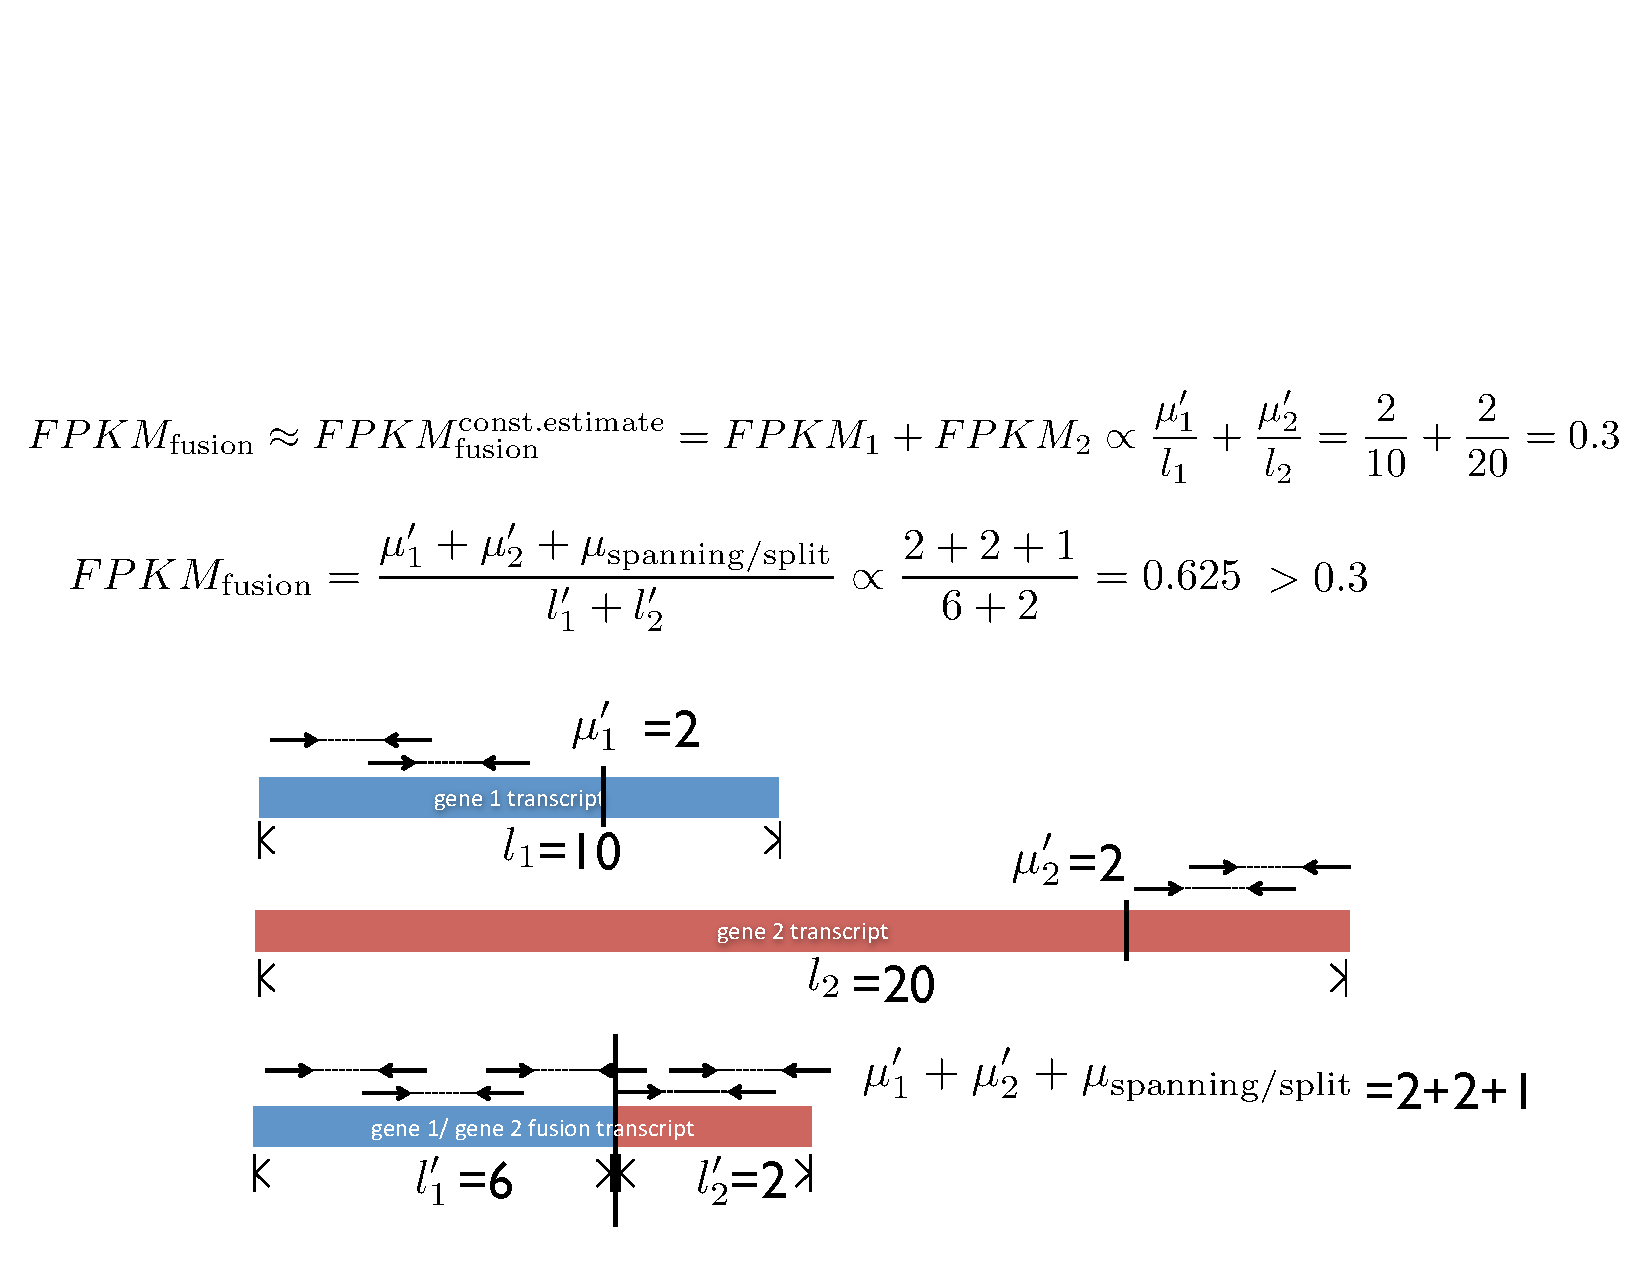
\includegraphics[width=.9\textwidth]{/Users/ijoseph/Documents/Work/Graduate-Thesis/TeX/figures/ch3_1.pdf}
    \caption{Illustration of inaccuracy of constituent summing method ($\mathrm{FPKM}_{\mathrm{fusion}}^{\mathrm{const.estimate}}$) for estimating expression of fusion transcript ($\mathrm{FPKM}_\mathrm{fusion}$), resulting in underestimation by a factor of $2$. $\mu_i \coloneqq$ number of reads aligning to transcript $i$; $l_i \coloneqq$ length of transcript $i$. $\mu_{\text{spanning/split}} \coloneqq$: sum of number of PRs and LRs.}}
\end{figure}
\end{center}


\subsubsection{Per-Exon Inspection}

A related but distinct method of assessing fusion genes is comparison between fusion-present and fusion-absent samples by visually inspecting the per-exon expression of the constituent transcripts. While not susceptible to the problems of the summing method in terms of misestimation, this is even more labor-intensive as it is completely not automated.

\subsubsection{Counting Junction-Spanning Reads}

One automated approach to assessing fusion expression estimation is by counting the number of reads supporting the fusion junction. In particular, a read can \textit{support} a fusion junction by being a \textit{spanning read} (PR) or \textit{split read} (LR). A PR is a paired-end read wherein one end maps to one transcript and another maps to a genomically distal genomic region, whereas an LR is a read wherein a portions of one read (if applicable) map to at least two distinct genomic regions.

Some method of counting these reads is a common method of prioritizing fusions; however, this is very susceptible to multi-mapping reads. In particular, if a junction region is repeated in another section of the genome, reads could spuriously seem to strongly support a fusion, whereas in reality the reads were produced by different regions altogether. Thus, this method can be inaccurate. One could imagine further difficult-to-set parameters describing heuristics for filtering these reads\cite{mcpherson_defuse:_2011}, but this is a complicated and error-prone process in and of itself.

\subsubsection{Problems with All Existing Methods of Fusion Expression Quantification}

With all of the above method, a fusions' expression is not directly comparable to the expression of other genes or transcripts. In particular, fusions' expression is not comparable to wild-type constituents' expression, which would be helpful in order to support functional activity of a fusion for prioritization and also for the existence of the fusion. Furthermore, none of the above methods are isoform-specific; all of these merely assess the expression of the fusion gene as a whole, even though isoform-specific expression has found to be impactful in cancer\cite{christofk_m2_2008}\cite{hovanes_-cateninsensitive_2001}\cite{_insulin_2003}.


\section{Method}

Thus, we propose an improved method for isoform-specific FG discovery and quantification from RNA-seq reads.

In short, the method involves three steps, all of which involve k-mer-based pseudoalignment methods: (1) discovering and aggregating LRs and PRs to predict FJs, (2) construction of candidate fusion transcript isoforms (CFTIs) from FJs, and (3) realignment of reads in order to quantify CFTIs along with all transcripts in the transcriptome.

\subsection{Predicting Fusion Junctions}

The first step of the method is to predict fusion junctions based on LRs and PRs. This is achieved using pseudoalignment methods, which in turn involve the splitting of reads into k-mers, the creation of a De Bruijn-graph transcriptome index for alignment, and aggregation of hashed alignment counts per equivalence class, each of which represent a subset of all possible transcripts.

First, reads with ends aligning to discordant equivalent classes are gathered as candidate PRs. Then, these are aggregated along with non-aligning reads (which include LRs) using a De Bruijn-graph alignment format to assemble candidate fusion junction regions. Finally, these regions themselves are pseudoaligned to the transcriptome in order to find candidate fusion junctions.

Note that this step can be replaced by the use of ordinary RNA-seq-read-based fusion finding tools, such as DeFuse\cite{mcpherson_defuse:_2011} or Tophat-Fusion\cite{kim_tophat-fusion:_2011}; results below show data generated by this method.

\subsection{Construction of Candidate Fusion Transcript Isoforms}

Given specific FJs in terms of genomic location, CFTIs are constructed based on enumeration of all possible unique isoforms downstream and upstream of this genomic region. These isoforms can then be added to the alignment index. Note that this can be a De Bruijn-graph-based transcriptomic index\cite{bray_near-optimal_2015} for pseudoalignment, or a Bowtie Burrows-Wheeler-based index \cite{langmead_fast_2012}.

\subsection{Estimating Expression of Fusion Transcripts}
Using the CTFI-appended transcriptome index, the classic generative-model based expression estimation approach is used to estimate the expression of all transcripts, including CFTIs.

Briefly, this model\cite{trapnell_transcript_2010}\cite{roberts_improving_2011}\cite{roberts_fragment_2013} operates via the estimation of parameters representing quantities of interest (transcript interest) and accounts for biases using other parameters, other parameters including per-transcript positional bias and read-composition-based sequence bias.

Importantly, this probabilistic model makes assumptions that assist with the recreation of transcript-wide, isoform specific expression estimation. Crucially, modulo the above biases, the uniform coverage assumption is used in order to deconvolute the extent to which non-junction spanning reads contribute to the expression of the fusion transcript.

The model is a likelihood-based approach which uses hidden data and the expectation-maximization\cite{tipping_mixtures_1999} algorithm to estimate parameters.

The result is an estimation of the expression of all transcripts in the CTFI-appended transcriptome, including, importantly, the CTFIs and their constituents.

\subsection{Checking for Impact of Fusion Transcript}

There are three distinct tests that can be performed for the related states of existence, expressional deregulation, and impact of a FJ and its candidate CTFIs:

\subsubsection{Overall increase in likelihood of model for including fusion transcript}

Since the probabilistic expression model gives a likelihood for a given set of transcripts and a given transcriptome, the likelihood for a fixed transcript set can be seen as a function of a transcriptome. The interpretation of this function is that it will take on a higher value of the transcriptome is more compatible with the sequencing reads; this can be seen as evidence that the transcriptome is the generating transcriptome.


Thus, the likelihood of the model can be compared between a transcriptome with and without CTFIs; this is direct evidence for the existence of a particular FJ and the related CTFIs.

\subsubsection{Decrease in bootstrap variance of constituents when including fusions}

Using the modern Kallisto\cite{bray_near-optimal_2015} expression estimation model, an empirical variance that represents the uncertainty of a particular transcript's expression is estimated. If these quantities decrease for the constituents upon addition of CTFIs, this can be also taken as evidence for FJ and CTFI existence.

\subsubsection{Test of nonzero expression for fusion transcripts}

Given the expression of all transcripts including CTFIs, one can validate the existence of a particular fusion transcript in a sample based on comparing the expression of the CTFI to the expression of its constituents. In particular, if the CTFI has high expression compared to each constituent, this can be seen as evidence for existence of the fusion transcript. However, if no CTFIs of a given FJ are expressed more than any of their constituent transcripts, this can be seen as evidence against the existence of that fusion transcript.

Regardless, this method allows for the identification of expressionally-deregulated fusion transcripts, in the sense that it allows for direct identification of expressional differences. This can be achieved via comparison of the fusion transcript's expression to the expression of constituents in a panel of matched normal cells known to be lacking the relevant FJ in their DNA. One can use formal differneital expression tools to gather significance for such a test, such as Cuffdiff or DESeq \todo{cite both}.

\section{Results}

In order to prototype and validate the method, we worked with members of the TCGA LGG AWG. In particular, collaborators at University of California, Santa Cruz and the MD Anderson Cancer Center both ran FJ-discovery software and prioritized samples and fusions for us to assess with our method.

\subsection{Overview of Group Findings}
The full analyses of LGG by the AWG were published in 2015 \cite{_comprehensive_2015}. The major findings, to which the above method contributed, were that there are three molecular categories of LGG that are effective at predicting prognosis. There was great concordance between sequencing datatypes in this regard. Thehe mutation status, obtained through somatic mutations, of the isocitrate dehydrogenase 1 (IDH1) gene plus the presence of chromosome arms 1p and 19q were sufficient to divide patients into three categories: IDH wildtype, IDH mutant with 1p/19q intact, and IDH mutant with 1p/19 deletions.

This was in concordance with clusters obtained via several unsupervised analyses based on DNA methylation, mRNA, copy number and reverse-phase protein assay. Thus, variance between patients ain the genome, epigenome, transcriptome, and proteome showed high concordance.

\subsection{Validation of Method}

Several fusions were detected using DeFuse\cite{mcpherson_defuse:_2011} and PRADA by collaborators in the group. These fusions were detected within IDH mutant samples and were investigated as possibly explaining within-group variation in prognosis based on known attributes of mechanism. One major category of fusions detected were those involving receptor tyrosine kinases, which are which are involved in cell signalling. As part of the mitogenic circuitry, activity of RTKs leads to mitotic cell division. RTKs are often activated via proximity; thus, overexpression is sufficient to induce activation, as it leads to a higher chance of proximity. 

\subsubsection{Case 1: FGFR3-TACC3 Fusion}

First, we studied a patient with a fusion detected between the Fibroblast Growth Factor Receptor 3 and the Transforming, Acidic, Coiled-coil-containing Protein 3 genes (an FGFR3-TACC3 fusion).

This fusion was a good candidate for validation of our method as it has been identified as undergoing fusion-modulated expressional deregulation \cite{parker_tumorigenic_2013}.

The mechanistic model is as follows\todo{figure from PDF at /Users/ijoseph/Documents/Work/Career/Applications/Roche-Sequencing/seminar.pdf}: the regulation of FGFR3 is based on the annealing of its 3' untranslated region (UTR) to a micro-RNA (miRNA) (miR-99a, in particular). When miR-99a anneals to the FGFR3 transcript, the transcript is marked for degradation. Thus, FGFR3's expression is downregulated based on its 3' UTR region. However, the fusion is formed such that the FGFR3 constituent lacks its 3' UTR, and therefore loses its wild-type regulatory mechanism. This leads to the temporally and spatially ectopically elevated expression of the FGFR3 sequence, leading to mitosis via mechanisms explained above.


Upon applying the method using eXpress as our expresion quantification module\cite{roberts_streaming_2013} on this specific paper, we were able to validate the results.

Firstly, we noted that isoforms of FGFR3-TACC3 fusion transcripts were among the highest-expressed transcripts in the transcriptome \todo{figure from page 38 of pdf}. This was a sanity check offering consistent evidence with the ectopically high expression of FGFR3-TACC3.


Secondly, we noted that we were able to differentiate between the expression of fusion transcript isoforms. In particular, we found that one isoform's expression dominated the expression of all others \todo{figure from 39 of PDF}.

Thirdly, we noted the correct assessment of the FGFR3-TACC3 fusion transcript isoform versus an FGFR3-AC016733.1 transcript, also formed based on the same FJ.

Finally, we validated that the expression of the fusion transcript was higher in expression than its constituents in the same cell \todo{figure from 40 of PDF}, finding that the fusion transcript's expression was more than 3 times the expression of FGFR3 and 100 times the expresion of the TACC3 transcript.

We also compared the fusion transcripts' expression to its constituents in matched normal tissue. This allowed for further evidence of the fusions' leading to expressional deregulation.

In order to make the comparison between the sample of interest and cerebral cortex samples from the Genotype-Tissue Expression project (GTEx)\cite{lonsdale_genotype-tissue_2013}, we transformed expression estimates from fragments per kilobase per million-reads-mapped (FPKM) to transcripts per million (TPM), then applied middle-50th-percentile-normalization \todo{cite what the FPKM}. We validated this normalization by using a housekeeping gene, heat-shock protein, 90-kilodaltons, alpha, class b, member 1 (HSP90AB1), for which strong evidence exists of relatively stable expresion temporally, spatially, and inter-cell-type. We saw that the expression in the sample of interest of HSP90AB1 was similar to that of the normal tissue.

We validated that the expresson of the highest-expression FGFR3-TACC3 fusion transcript isoform was much higher than that of its constituents the matched normals -- on the order of 10 to 1000 times higher.

\subsubsection{EGFR-SEPT14 Fusion}

We also studied a fusion between the epidermal growth factor receptor (EFGR) and septin 14 (SEPT14) genes (EGFR-SEPT14 fusion). EGFR is another RTK with similar activity to FGFR3, and was thus another candidate for a fusion having similar oncogenic properties to the FGFR3-TACC3 fusion, although unknown in its ability to expressionally deregulate. EGFR3-SEPT14 is also known to have oncogenic properties in glioblastoma, which is equivalent to grade IV glioma and related as a progression result to LGGs \todo{OMIM entry HEAT SHOCK}.

Once again, we noticed that the expression of the fusion transcripts were above their constituents in many cases \todo{insert figure from supplement of NEJM}. This suggests expressional deregulation occurred for this fusion.

\section{Discussion}

\subsection{Outlook}
The validation of a known expressionally-deregulated fusion and the identification of a candidate expressionally-deregulated fusion is promising that the method will be useful at identifying expressionally-deregulated fusions in the future based on the metric of assessing the expression of the fusions to be significantly higher than their constituents.

\subsection{Future Work}
  
Much future work could be done on this method; firstly, one could create a formal statistical test of the expression of a fusion transcript being higher than its constituents (a) within sample and (b)a matched panel of normals. This would expedite the identification of expressionally deregulated fusions and would complete the requirement for not requiring manual user assessment of results.

Secondly, one could expand on this method to both identify FJs and lead to their expression. Currently, this is being done by Shannon Hateley and Dr. P\'{a}ll Melsted, Ph.D. by adapting the Kallisto pseudoalignment algorithm\cite{bray_near-optimal_2016} to identify FJs based on discordantly-mapped k-mers.

Thirdly, one could also use modern k-mer-mapping-based expression methods to achieve the expression quantification portion, which are much faster and would be useful as well for providing variance-based evidence for fusion existence.

Fourthly, one could integrate this into one tool, such that pipelining, which is a tedious and error-prone process, would not have to be implemented by the user.










\chapter{Integrating genomics data for prediction, with application to gliomas}

\section{Background}

One specific prediction problem in gliomas, specifically LGGs, is related to response to chemotherapy. Currently, there is no suggested guideline, according to the World Health Organization and no standard practice between care centers as to whether or not to give chemotherapy following initial resection of the primary tumor in LGG patients.

In particular, temozolomide (TMZ) is given to about 50\% of patients being given TMZ following 
primary therapy. Confounding this decision is the recent finding by Johnson et al. that TMZ appears to be inducing mutations in certain patients which may increase the severity of the recurrent tumor in terms of grade. 

However, it is possible that high-throughput (HT) genomic data might be able to assist in this treatment decision-making problem via predictions. Empirically, several survival time-related HT features have been identified by TCGA; since some of these patients have been treated with TMZ, it is possible that said molecular features might inform recurrence grade decisions for these patients as well, since recurrence grade is associated statistically with survival time. 
Molecularly (theoretically), the mechanism behind TMZ-induced greater recurrence is partially known.

\subsection{Candidate molecular mechanism}
In particular, TMZ induces cytotoxicity by inducing nuclear genomic mutations, which then cause cells to induce apoptosis. In particular, TMZ adds a methyl group to (methylates) guanine bases in the genome, creating an adduct. The adducts lead to recognition during replication by MMR genes, which recognizes the resulting mismatches but then repeatedly attempts to repair the region ineffectively by reinsertion of the incorrect base, leading to genomic double-strand breaks and apoptosis. 

This apoptosis of quickly replicating tumor cells is the desired effect of TMZ. However, there are several reasons why this might not occur, due to other potentially extant yet testable genomic changes.

Firstly, if apoptotic cell cycle checkpoint machinery is not functioning normally, this leads to consequently genomic instability and large-scale structural rearrangements.  Secondly, TMZ-created adducts are removed by MGMT if available and functional. However, if MGMT has a promoter region that is itself methylated, this leads to decreased MGMT expression and persistence of the TMZ-added methylation adducts beyond that which is normal, leading to increasing numbers of mutations possibly beyond even wild-type MMR machinery’s ability to detect and control. 
These two potential issues with TMZ-related apoptosis are thought to be related to the hypermutation phenotype (quantified by much higher mutations per base rates than other tumors), which is correlated with the recurrence as high-grade. Evidence for this is based on TMZ-related mutational patterns having been observed in tumors with hypermutation phenotypes, and the existence of these patterns in regions relating to the above machinery.

\section{Problem formulation}

Underlying this prediction problem in abstraction is a prediction problem: in particular, given high-dimensional clinical and molecular data, can one predict, for a particular patient, whether TMZ-induced hypermutation will occur?


Finding associations can be generalized as a prediction of one random variable $y$ from another, $\vec{x}$, by a function $f$. The goal is to estimate $f$. $f$'s performance can be assessed by expected predicted error from true $f$, which is a function of the complexity of $f$. $f$'s complexity raises with the dimensionality of its input $\vec{x}$, which leads to an estimate of $y$ that has high variance, which confounds interpretation of any one association as being significant.

In order to address this issue, smoothing parameters can be added to $f$ in order to decrease the variance of $f$; these are tantamount to making specific assumptions about the underlying probabilistic model that generated the data, which can, in turn, bias the estimate of the 
association. However, this may still lead to an overall reduction in the expected predicted error, which is a function of both bias and variance of $f$.


One of the model assumptions that we make is linearity (specifically, that $f$ uses first-order linear terms to manipulate $\vec{x}$ for performing predictions of $y$, which is a common assumption \cite{friedman_elements_2001} useful for simplification of $f$. This is implemented by linear dimensionality reduction techniques – specifically, the factor association analysis (FAA) method.

\subsection{Heterogeneity challenge}

A fundamental challenge with this prediction problem is the heterogeneity of data types involved the prediction problem. In particular, there is molecular data which may include germline variants of various forms detected by various different exome sequencing pipelines, gnomic copy number data based on arrays and/or DNA-sequencing, expression detected by a RNA-seq and/or microarray platforms, methylation detected by microarrays and/or sequencing-based techniques, and uni-dimensional clinical covariates. 


In particular, this will manifest as different underlying distributions that best approximate each data type, both between patients within a specific modality (due to heterogeneity of platforms) and between modalities within a specific patient.


\subsubsection{Unsupervised solutions}

Unsupervised machine learning approaches, which seek to more clearly represent variances in a dataset without any explicit inclusion of specific outcomes of interest, have been used to assess multi-platform genomic data.

\begin{description}
\item[Consensus clustering]
  \textit{Consensus clustering} or \textit{cluster-of-cluster} \cite{kristensen_principles_2014-1} methods combine datatypes by hierarchically clustering samples within each datatype, then using the specific cluster assigned per data-type as a feature for a meta-clustering approach. This is best used successfully in situations where variance is shared among multiple different genomic datatypes, \textit{and} that shared variance is mostly or largely a component of the outcome of interest. This was used by collaborators at UCSF as part of the TCGA LGG AWG \cite{_comprehensive_2015}, where shared variance across datatypes was associated with survival time.

\item[factor analysis-based approaches] Approaches such as iCluster \cite{shen_integrative_2012}\cite{shen_integrative_2009} use an explicit probabilistic generative model in order to reduce dimensionality and simultaneously find shared variance among a different number of sequencing datatypes, allowing for parametric assumptions useful for sequencing data type distributions (for example, modelling mutation calls as Bernoulli random variables). This approach has not been heretofore expanded into a supervised setting.

  
\item[PARADIGM]
  PARADIGM models explicit interactions between sequencing datatypes using existing models of gene interaction networks as well as assumptions about functionality \cite{vaske_inference_2010} \cite{ng_paradigm-shift_2012}. In particular, the activity of every gene is predicted based on the status of its corresponding copy number, mutation status, and gene expression, assuming, for example, that a deleted gene should not be functional, or a gene that is mutated but is not expressed should not be directly functional.
  PARADIGM effectively reduces high-dimensional datasets to inferences about the activity level on a per-pathway basis for further manual investigation. 
  PARADIGM suffers from a wealth of parameters, and therefore necessitates a relatively large amount of data to prevent overfitting.   
\end{description}

One limitation of all unsupervised approaches is the necessity of the outcome of interest to correspond to the shared variance among the sequencing datatypes, which may not be the case. This is addressed by supervised methods. 



\subsubsection{Supervised solutions}

Many supervised approaches merely add features from multiple platforms without specific inclusion of special related assumptions into the model.

This is appropriate for some models, for example, random survival trees, which are robust to different feature distribution assumptions.

This is less appropriate for linear models. Thus, a few linear supervised machine learning models have been created in order to address the use of heterogeneous sequencing data types as features in order to predict an outcome of interest. This is an area of intense current research.

\begin{description}
\item[regression on residuals]
  Yuan, Allen, and Omberg et al. \cite{yuan_assessing_2014} looked at the improvement from adding single molecular datatypes to a clinical variable model of predicting overall survival time in four cancer types with data from TCGA, using a cox multivariate proportional hazards model. In particular, after regressing out the predictive clinical information from the feature set on the outcome, individual genomic features were selected by choosing those that explained the residual variance in the survival time outcome, and added as regular features to the model. However, this was not found to be more accurate than merely using the additional features in random forest models without any special annotation of sequencing data types.  


\item[canonical correlation analysis-based approaches]
  Canonical correlation analysis, which is originally an unsupervised technique to find shared variance between two feature sets, has been adapted into supervised models by adding an outcome of interest \cite{shen_novel_2014} \cite{bair_prediction_2006}\cite{yu_supervised_2006}\cite{witten_extensions_2009}. This was used with some success by Drs. Robert Tibshirani and Samuel Gross as a predictor for diffuse B-cell lymphoma prediction of copy number. Recently, an extension was proposed: the \textit{Collaborative Regression} method\cite{gross_collaborative_2015}. This method addressed shortcomings of previous methods by formulating the problem in a way that is convex, and therefore algorithmically efficient.

  However, these methods were not specified probabilistically, and therefore are not as amenable to extensions involving explicit data type distribution specifications. In addition, the adaptation of CCA used above was approximate, and thereby is possibly less statistically powerful than a precise (probabilistic) specification. Furthermore, not being probabilistic, these models cannot be used generatively, preventing them using simulation to assess model performance parameters, such as requisite $N$, $p$, and effect size. 
  
\end{description}


\subsection{Dimensionality challenge}
A perhaps bigger fundamental challenge with this prediction problem is what is referred to as “the curse of high-dimensionality,” that is to say, there are many more covariates/predictors ($\text{number of predictors} \coloneqq p $) than observations ($N$) (i.e., $p \gg N$).  This is inherent to this problem due to the wildly high-dimensionality of the molecular datasets, which at their current maximum for even a single modality is about $500,000$ with reasonable granularity, but could theoretically be on the order of $10^9$. This is manifests as an issue by leading to overfitting or equivalently, high variance in estimators of associations.

Fortunately, these problems are not unique to this particular prediction problem, and consequently, several techniques have been developed to deal with both of these fundamental challenges. 

\subsubsection{Subset selection approaches}

Subset selection involves using only a subset of available features, which must be selected. There are several methods for doing so in order to address the exponential number of possible subsets, including forward and backwards stepwise regression, which iteratively adds or removes predictors based on relationship to the outcome. However, these methods suffer from relatively high prediction error due to the high variance imposed by the discrete inclusion or exclusion of a specific parameter\cite{friedman_elements_2001}.

\subsubsection{Shrinkage approaches}

A standard method of addressing high-dimensionality and related high variance of any estimated fit parameters that stymie attempts to generalize is by adding a model term that explicitly adds a penalization on the use of each parameter. An optimization is then performed over this adjusted function. Relatedly, a constraint can be placed on the size of the features and solutions within a particular constraint can be sought. Parameters involving the degree of regularization are selected based on a \textit{model selection} step, which typically attempts to assess the expected prediction error of a model with several different parameter settings in order to identify the most accurate combination. 

The specific penalty that is applied to each feature may be \textit{Lasso}, which uses the $L1$-norm of the vector of coefficients: $\sum_{j=1}^p | \beta_j | \leq t$, where $\beta_j$ is each coefficient on the $p$ parameters, and $t$ is a pre-specified constant. Another common approach is \textit{Ridge}, which uses the $L2$-norm of the coefficient vector:  $\sum_{j=1}^p  \beta_j^2  \leq t$. These have different properties, with Lasso generally leading to more sparsity. However, this may be an incorrect assumption that hurts generalizability; to address this, \textit{Elastic Net} regression was created, which involves a hyper-parameter that is specified to address the relative contribution of ridge and lasso constraints. 


\subsubsection{Dimensionality-reduction approaches}

Dimensionality-reduction approaches offer a natural method of dealing with large numbers of correlated features -- modeling the high dimensionality of these features by a small number of independent features, and using these as new prediction features. Approaches such as \textit{principal components regression} and \textit{partial least squares} achieve this.

However, existing dimensionality reduction techniques typically do not also directly address heterogeneity in the feature space. 



\section{Developed method}
\subsubsection{Inspiration from unsupervised dimensionality reduction models}

This method’s development came about due to the observation by Novembre and Stephens\cite{novembre_interpreting_2008} that when taking the principal component analysis (PCA) of the single nucleotide variants present in individuals, the first few components correlated highly with geographic location of the individual. Briefly, PCA finds a ranked list whose entries consist of linear combinations of variables that explain decreasing components of the variance in a given matrix; in this case, that matrix $\mathbf{V}$ $(\text{people } \times \text{genomic\ variants})$.

Novembre’s result can be interpreted as much of the first two statistically independent sources of variance in the common gene variants ``explains'' their geographic location. This knowledge can then be used to decrease geographically-related variance in the germline variants of patients in GWAS studies, increasing their statistical power by decreasing noise.


Recently, gene expression information has also begun to be collected on a large sale, enabled by recent decreases in technology price. Dr. Lior Pachter, Dr. Nicholas Bray, Brielin Brown, and Dr. McCurdy consequently wondered if gene expression information also contained significant geographic signal, and consequently performed PCA on the gene expression matrix $\mathbf{G}$ $(\text{people} \times \text{genes})$. However, the first few components did not correlate directly with geography.


This then led to the application of canonical correlation analysis (CCA) to this dataset in order to directly find shared variance between the two-dimensional geographic origin ($\mathbf{R}: \text{people} \times (\text{latitude}, \text{ longitude}$)) of the individuals and their high-dimensional associated gene expression vector (i.e., CCA between $\mathbf{G}$ and $\mathbf{R}}$). Briefly, CCA is analogous to PCA, except for linear combinations are taken of both matrices (termed ``canonical functions'' (CFs)) instead of just one matrix, and they are taken in ways that maximize the correlation between the linear combinations of one matrix with the other. The first two canonical components (CCs) in the above analysis therefore, by construction, should have significant correlation with the geographic coordinates, at least inasmuch as the component on the geographic matrix.


This was indeed found to be the case; however, it was quickly realized when doing permutation testing that the $p \gg N$ issue resulted in overfitting (i.e., no CFs were statistically significant), due to the high dimensionality of $\mathbf{G}$. This was addressed with a specific type of regularization. In particular, $\mathbf{G}$'s dimensionality was first reduced using PCA to $\mathbf{G}'$, and then CCA was performed between $\mathbf{G'}$ and $\mathbf{R}}$, resulting in statistically significant CFs. Visualization of these then revealed the desired correlation with geography.

\subsubsection{Formulation based on PCA and CCA}

Out of this was borne an inspiration to use a probabilistic model to create more nuanced dependency relationships between various datatypes.


PCA\cite{tipping_probabilistic_1999}, which can be interpreted as probabilistic graphical model with a latent variable emitting an observed variable based on a dimensionality expansion plus diagonal noise.

CCA can be viewed as a dimensionality reduction technique similar to PCA the sense that both matrices are reduced in dimensionality such that they correlate most with one another. One can also, relatedly, formulate CCA probabilistically as finding a maximum likelihood solution for a probabilistic general model in which a low-dimensional latent space expanded into higher dimensions with added noise of a specific structure -- positive semidefinite noise and with two observed variables. Thus, some combination of these two (PCA and CCA) noise constraints was indicated in order to simulate the PCA/CCA combination above in a probabilistic fashion.

One way that these can be combined in a probabilistic model is through simply adding an intermediate node between the observed data and the latent data, and have the intermediate node be generated from the latent node with diagonal noise, and the observed node be generated from the intermediate node with positive semidefinite noise.

As a generalization to more than two datatypes, one can imagine recursively applying this, such that, for example, if $\mathbf{G'}$ and $\mathbf{R}}$ are predicted to have been generated from $\mathbf{H}$, a lower-dimensional space, and then performing FAA on $\mathbf{H}$ and $\mathbf{S}$ to find $\mathbf{T}$, etc. We define this as a hierarchical factor association model (HFAM). This lends FAA to more complicated association problems than merely two datasets with two datatypes.

This successful application of HFAM in geographic explanation of gene expression setting and the recognition of its non-setting-specific theoretical nature as a framework led to the idea of applying it in other datasets, in particular those in cancer genomics in prediction problems. 
Thus came the inspiration for applying it to the prediction problem related to severity of recurrence upon application of TMZ given several HT genomic datatypes.


\subsubsection{Formal model specification}
In more concrete terms, the proposed HFAM consists of a latent factor model with $n_z > 1$ latent multidimensional variables $\z_1,... \z_{n_z}$ and $n_x >1$ observed variables $\x_1, ..., x_{n_x}$.

$\z_1$ is taken to be generated by a normal prior wtih identity variance: $\z_1 \sim N(\0, \mathbf{I})$

Variables are generated from other variables as follows: ${\vec{\gamma}}$ is a dimensionality expansion of $\vec{\delta}$ , plus noise:  $\vec{\gamma} \sim \W _\gamma \vec{\delta} + \vec{\epsilon}_\gamma$. $\vec{\epsilon}_\gamma \sim N(\vec{0} , \bpsi_\gamma)$, where $\bpsi_\gamma$ can be specified to be diagonal or unconstrained. We are using the normal distribution $\vec{\gamma} \sim N(\W_\gamma \vec{\delta}, \bpsi_\gamma)$, although other distributions could be used as an extension.

One specific observed variable is set to be the outcome of interest: $\x_i \coloneqq \y$. 

In general, observed variables are specified to have diagonal noise in their generation from latent variables, whereas latent variables are specified to have unconstrained noise in their generation from other latent variables (other than $\z_1$). 


As a graphical model, this can be viewed as a multifurcating tree, with root $\z_1$ and leaves $\x_1, ..., x_{n_x}$, where an arrow from $\delta$ to $\gamma$ indicates the relationship outlined above. As an example, see an instance of the model with three observed nodes and two hidden nodes ($n_z = 2, n_x = 3$) (figure \ref{threenode}).

\begin{figure}
  \centering  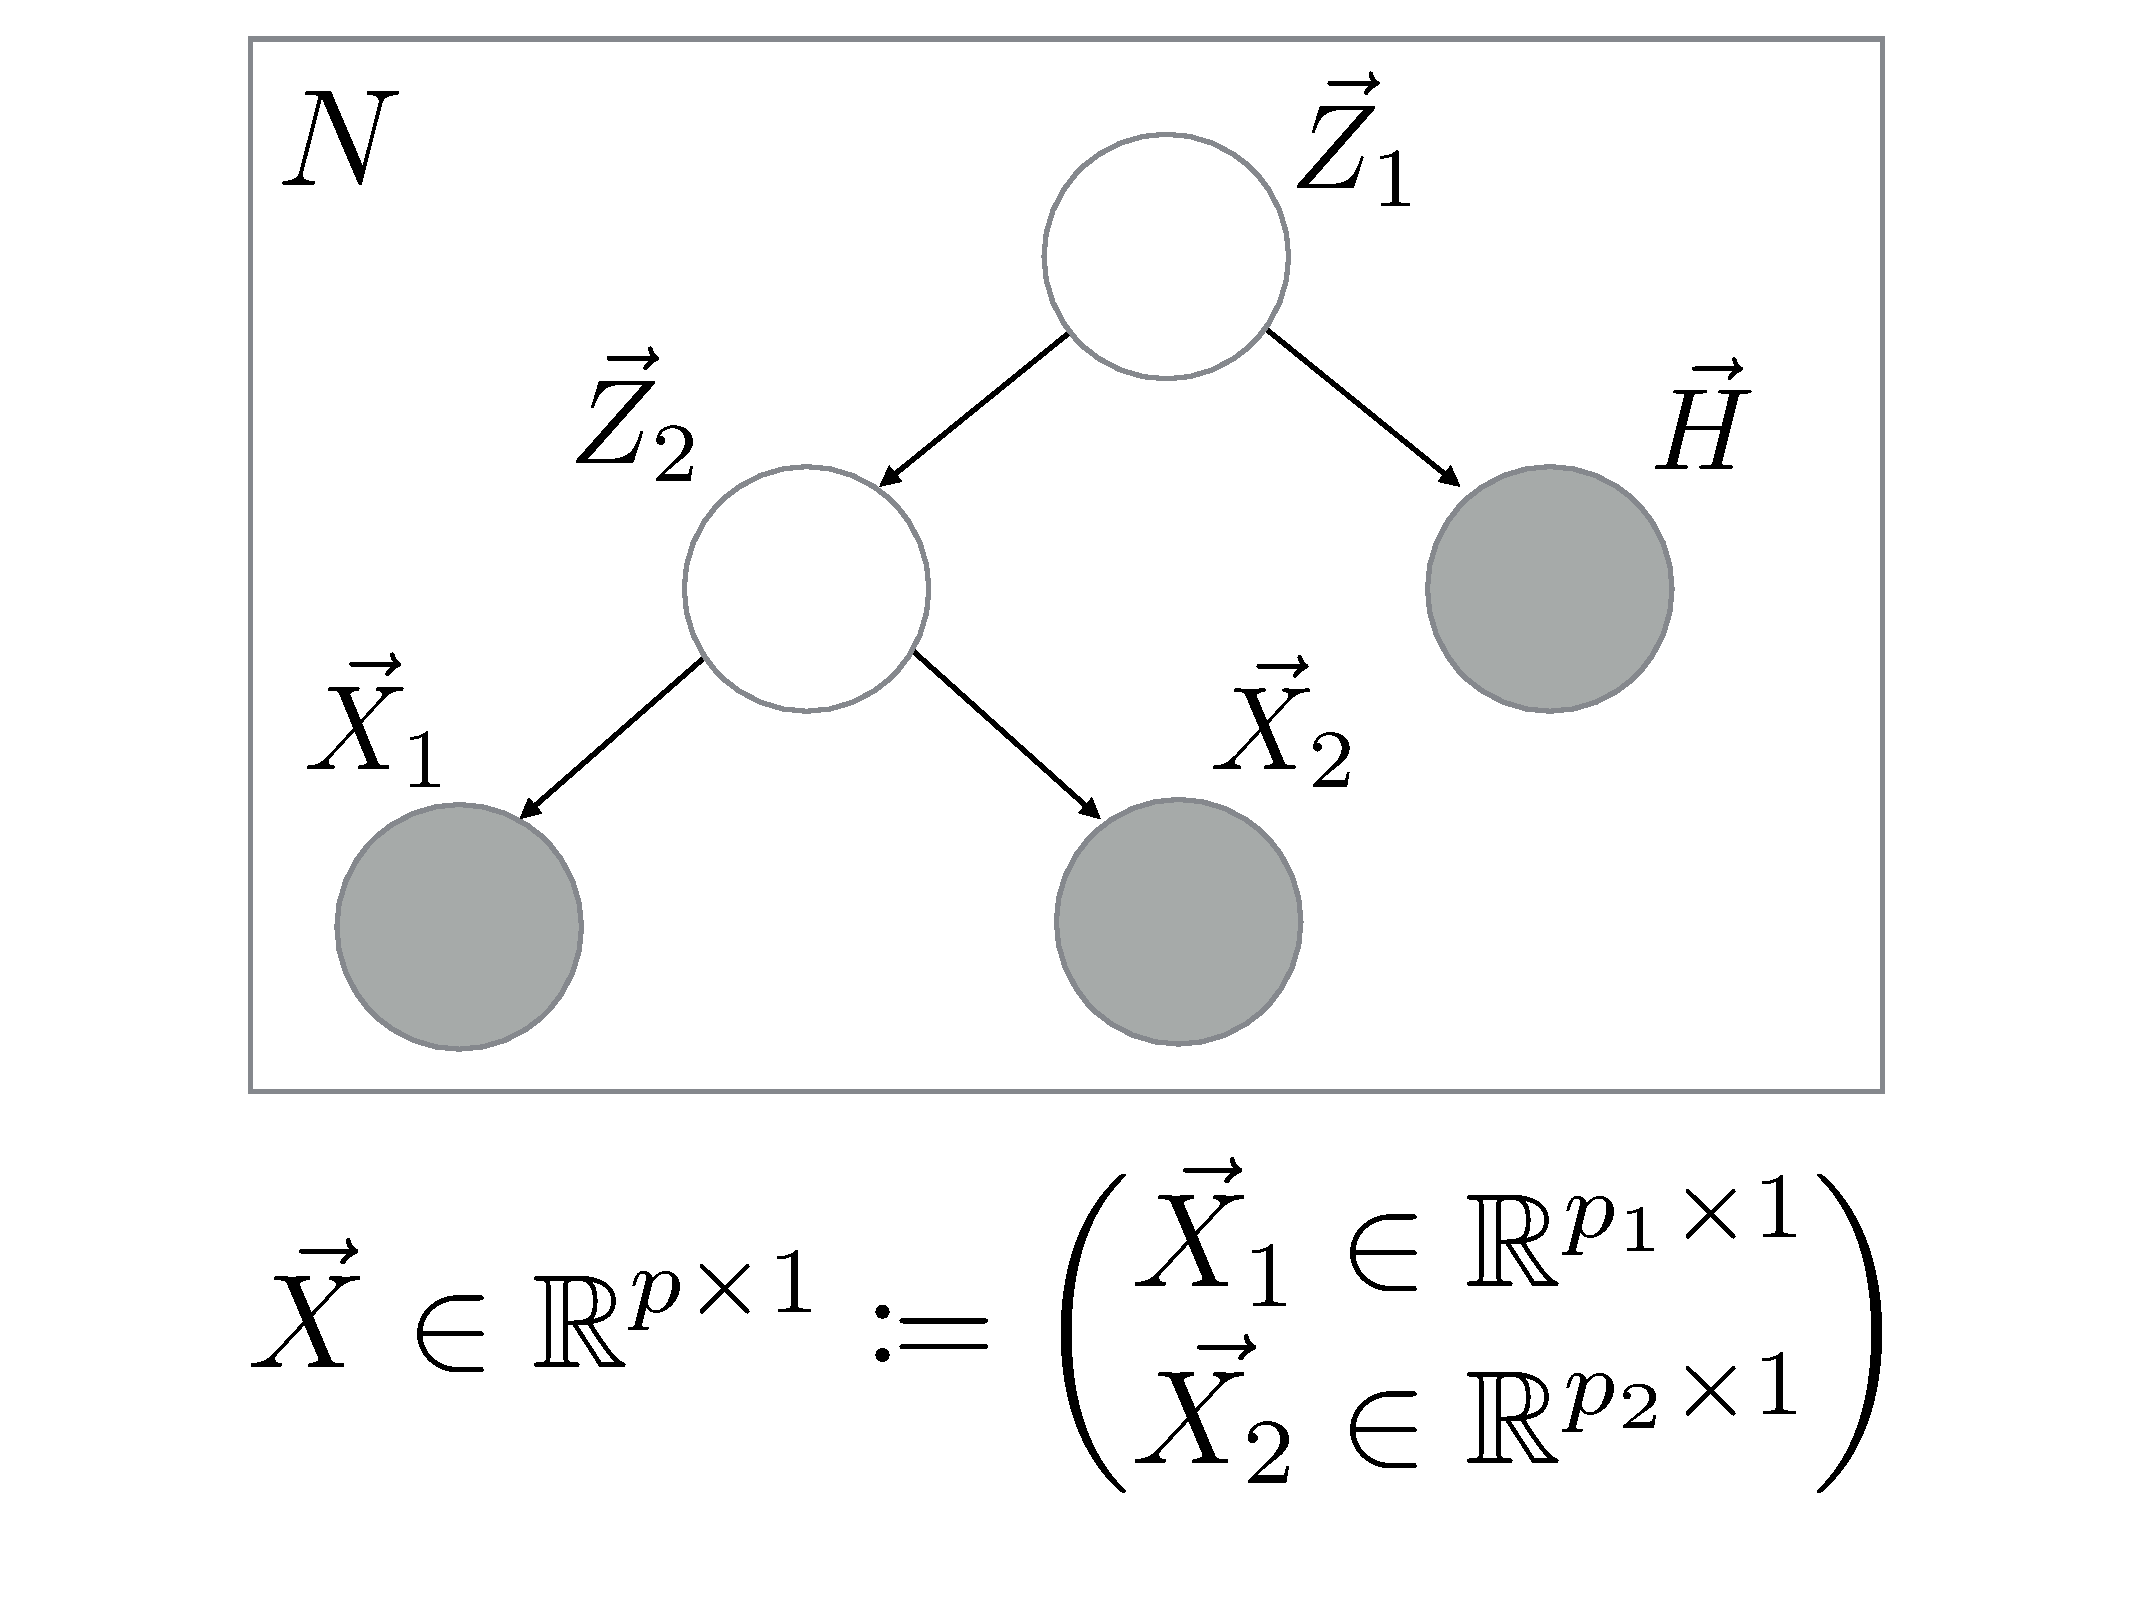
\includegraphics[width=.9\textwidth]{/Users/ijoseph/Documents/Work/Graduate-Thesis/TeX/figures/ch4/threenodemodel.pdf}
      \caption{Three-node HFAM. Here our outcome $\vec{y}$ is represented by $\vec{H}$.} \label{threenode}
\end{figure}


This model can be seen as imposing a specific structure on the covariance matrix of the data which is appropriate for the supervised modeling of sequencing data towards a specific response. In particular, it imposes a block joint covariance structure. See appendix for an example.  

Inference is done using the expectation-maximization (EM) algorithm in order to estimate the parameters: $\bTheta \coloneqq \left\{\W_i, \bpsi_i \right\}_{i=1}^{n_x + n_z}$ as well as the latent variables $\z_1,... \z_{n_z}$. See the appendix for EM parameter updates derived for a three-node model. 


After learning parameters $\bTheta$, one can predict $y$ from input observed variables. See the appendix for details.

\subsubsection{Consistency of model structure and genomics assumptions}

The above model specification if used with one multifurcating second-level latent variable and one high-level latent variable of relatively low dimension induces model assumptions we feel are consistent with reasonable assumptions for the datatype, and simultaneously address the challenges of heterogeneity and high-dimensionality. In particular, dimensionality is addressed through the use of relatively low-dimensional latent variables $z_i$ -- on the order of $10^0$ in our simulations and $10^1$ on CGP data.

Heterogeneity is handled as follows: when diagonal noise variances are used for observed variables, this forces covariance within-feature set to be reflected in the latent variable and consequently sibling variables; thus, the latent variable can be seen as storing covariance that is both within-feature type and between-feature type. This is reflected in the associated variable $\W$. In addition, the multi-level hierarchical nature with unconstrained variance between the latent nodes leads to a variable amount of shared-sequencing variance to be used to explain the outcome of interest.

This is consistent with intuitive and established notions about empirical shared variance between sequencing types and outcomes: \textit{some} of the shared variance between shared data types will be relevant for the outcome, but not all. It can also be seen as using each additional sequencing datatype as further evidence for a particular variance structure. It differs from a single latent-node model, which will expect all covariance within feature-datatype to be explained in the outcome variable. This  can be seen using Bayes' ball approach for studying dependencies in probabilistic graphical models (see \ref{foursix}).


    \begin{figure} 
      \centering
      \subfloat[][Bayes' ball shows shared variance between observed features but not outcome  possible]{\noindent
        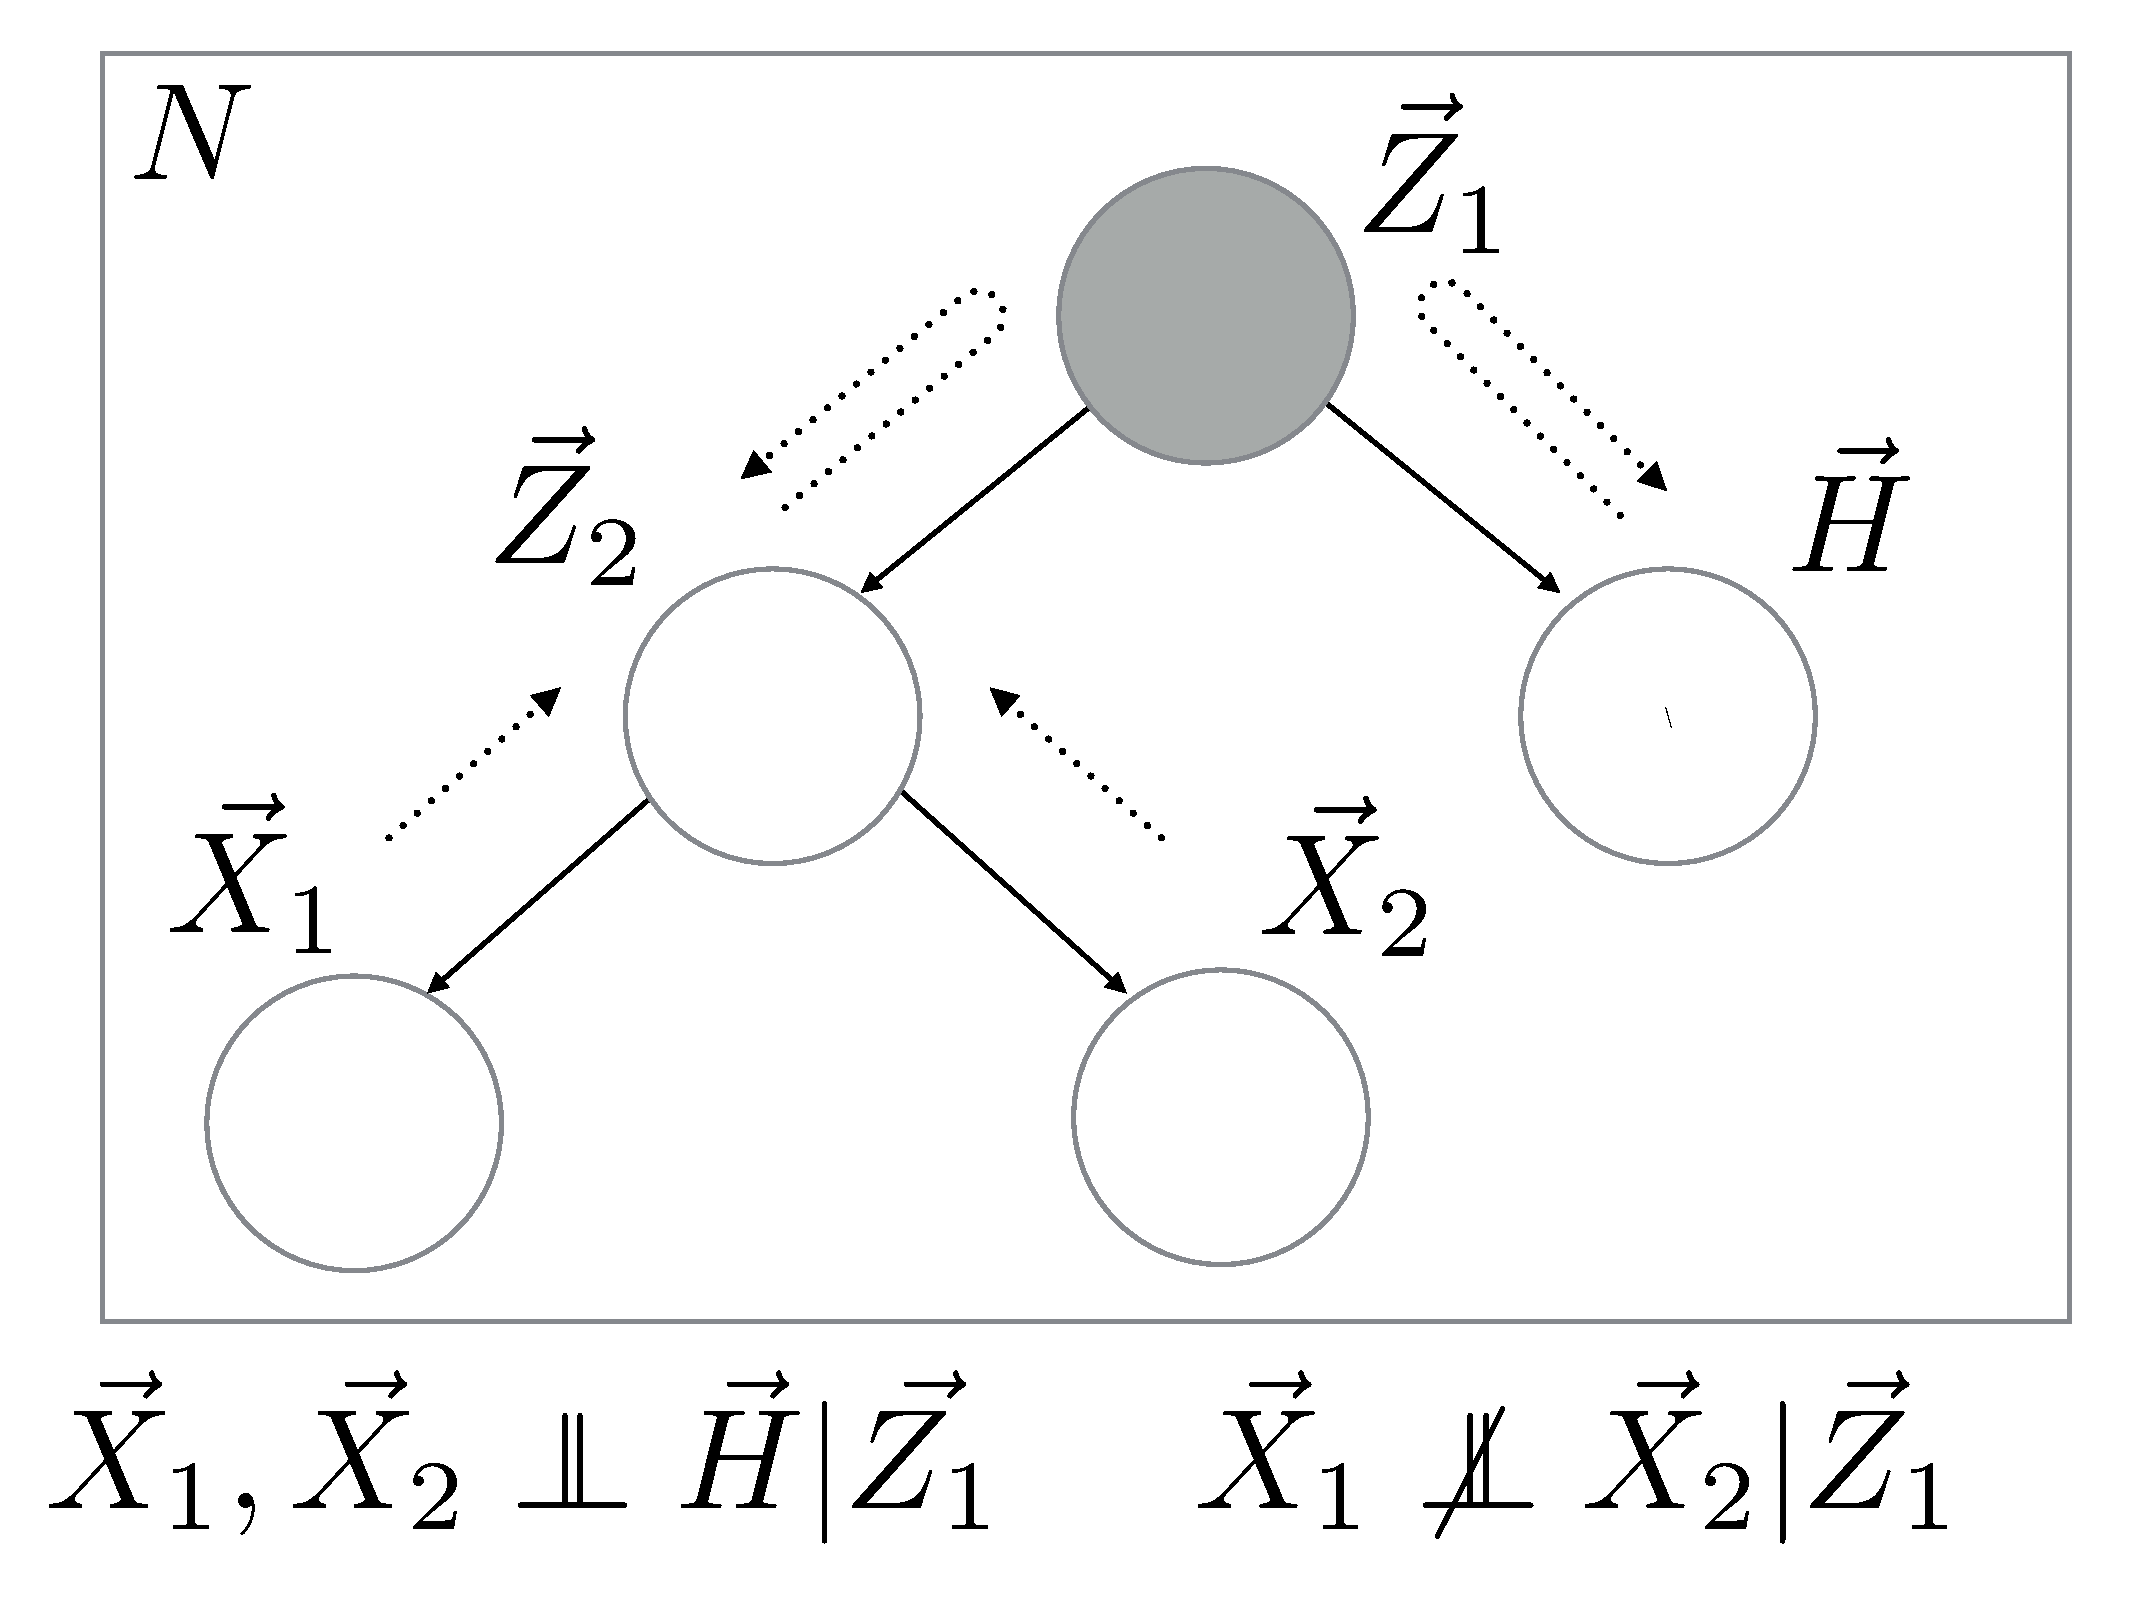
\includegraphics[width=.4\textwidth]{/Users/ijoseph/Documents/Work/Graduate-Thesis/TeX/figures/ch4/bayesball1.pdf}}%
      \qquad \\
      \subfloat[][Bayes' ball shows that shared variance between observed features must also be between outcome ($\vec{H}$)]{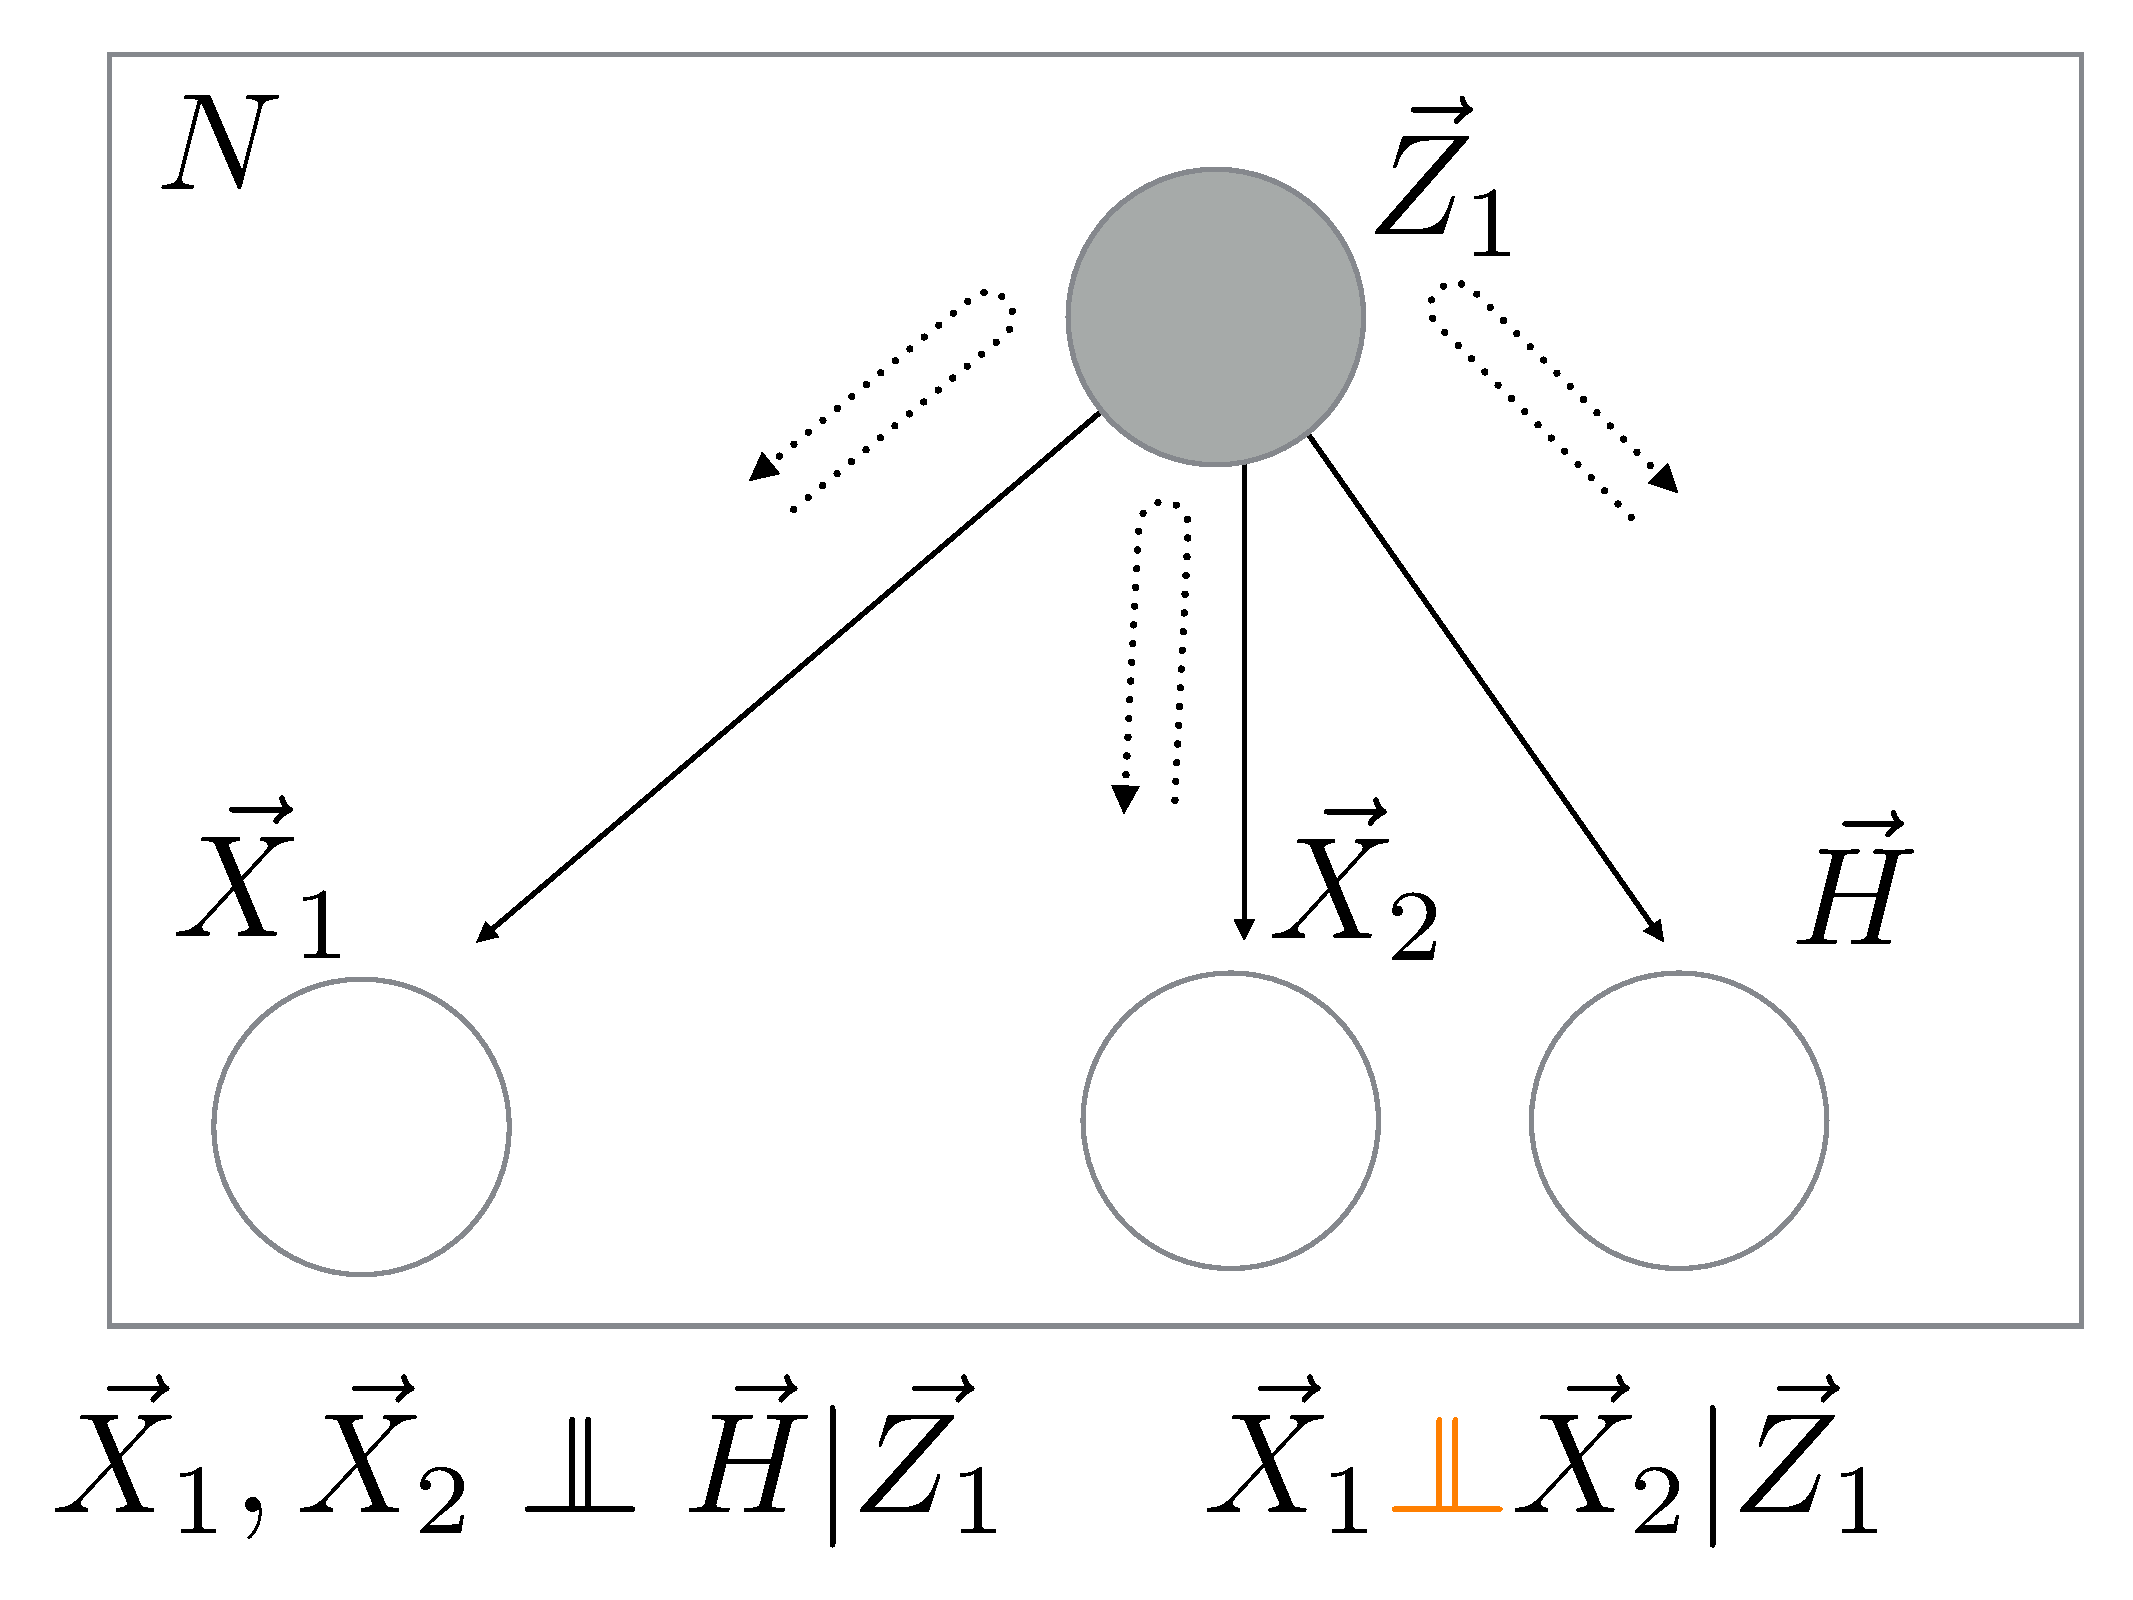
\includegraphics[width=.4\textwidth]{/Users/ijoseph/Documents/Work/Graduate-Thesis/TeX/figures/ch4/bayesball2.pdf}}%      
      \caption{Bayes' ball depiction of difference of hierarchical model layout} \label{foursix}
    \end{figure}



\subsubsection{Implementation}

The above model was implemented with a set of \texttt{python} classes and associated script. It allows for the specification of a general-structure model and its parameters (number of nodes, their associated dimensions, and the diagonal or non-diagonal variance structure of noise). See \href{https://bitbucket.org/ijoseph/factorassociationanalysiscancergenomics/}{the \texttt{Bitbucket}\reg repository} \\ (\url{https://bitbucket.org/ijoseph/factorassociationanalysiscancergenomics/}) for details.

Briefly, the \texttt{GaussianLatentFactorModel} class includes logic for inference and prediction, and \texttt{ThreeNodeGaussianModel} shows an example of a three-node implementation with minimal specification.

\section{Results}
We present the results on three different datasets of increasing difficulty: (1) simulated data with arbitrary parameters, and in order to discover necessary parameters for accurate prediction, (2) data from the Cancer Genome Project\cite{ledford_end_2015} with around $1,000$ samples and $100,000$ features, and the Costello Lab (see chapter 2 for details of all).

\subsection{Assessment}

Machine learning assessment is a rich field, with many options available.

\subsubsection{Expected prediction error motivation}

Essentially, one important metric to measure is \texit{expected prediction error}, which describes the expected accuracy of a given fit model on predicting from data arising from the same distribution under which it was trained \cite{friedman_elements_2001}.

Under situations with unlimited data size and resources, one would estimate this by using a training/ validation/ test split of the available data, where $50\%$ of the data is used for training, $25\%$ is used for validation, and another $25\%$ is used for testing.

The \textit{training} set would be used to fit the model. The \textit{validation} set would be used to estimate the expected prediction error for a given setting of model tuning parameters (related to model complexity and therefore tendency to over or underfit). Different tuning parameters would be assessed until one with acceptable expected prediction error were found on the validation set. The \textit{testing} set would be used to confirm the expected prediction error.

However, under a relatively limited number of samples, one might perform \textit{cross-validation} in order to assess the prediction error from a limited number of samples. This eschews the need for a validation set, and estimates one based on iteratively holding various small subsets of the data and assessing prediction error on the small subsets.

For expediency and data-size reasons, we chose to use cross-validation in this manner in order to estimate prediction error.

Practically, we assessed the below performance by interfacing with \texttt{scikit-learn}\cite{pedregosa_scikit-learn:_2011}, a package with built-in assessment tools, and also used existing machine learning models in this package for comparison. 


\subsubsection{AUC metric}
For a given set of predictions on data, one can assess accuracy based on the \textit{area under the [receiver-operating characteristic (ROC)] curve (AUC)}, a common measure of classifier efficacy\cite{friedman_elements_2001}. Briefly, the ROC curve's axes specify the particular specificity achievable for a given setting of sensitivity. An AUC of $1$ indicates perfect classification, whereas $0.5$ indicates a classifier that is no better than chance.

\subsubsection{Confusion matrix}
In order to complement the ROC curve and AUC, we also studied \textit{confusion matrices} based on cross-validation predictions, which show, for a given fixed sensitivity/specificity, the number of true positives, false positives, false negatives, and true negatives.

\subsection{Simulated data} 

We sought to validate that the model was performing as expected, and also to assess the necessary effect size for a given setting of $N$ and $p$. Effect size was approximated through the setting of a specific parameter of element-wise average $\mathbf{e} \coloneqq \frac{\W}{\bpsi}$ for parameter generation, where a larger setting of this quantity indicated higher signal-to-noise ratio and effect size. In essence, this means that the latent variables of the model explain more about the association between the datatypes than the noise specific to each datatype.

For simulations, we chose the dimension of $z_1$ to be $2$ and $z_2$ to be $3$. For logistic regression, we set left the Lasso regularization strength at $C=1$, its default.

Since we are interested in a classification problem and the model as specified generates floating-point numbers as observed data, we made the additional step of binarizing one of the one-dimensional output nodes based on the empirical mean of the simulated distribution. 


\subsubsection{$\mathbf{p \ll N}$}

First, we sought to assess whether the model would lead to more accurate recovery of its simulated data than other models. We chose logistic regression with lasso penalty as a model for comparison.

\begin{description}
\item[$\mathbf{N=1,000, p=10}$] We used $N=1,000$ and $p=10$
  ($n_x = 3$, with two $5$-dimensional feature nodes). $N=1,000$
  corresponds to the approximate number of samples in the Cancer
  Genome Project\cite{ledford_end_2015} dataset.

  We found that the model was slightly superior from an AUC
  perspective, especially with relatively low effect size
  ($e \leftarrow 1.25$).See figures \ref{fourthreeone}, \ref{fourthreetwo}, \ref{fourthreethree}, \ref{fourthreefour}.
    \begin{figure} 
      \centering
      \subfloat[][$e=1$.]{\noindent
        \includegraphics[width=.4\textwidth]{/Users/ijoseph/Documents/Work/Graduate-Thesis/TeX/figures/ch4/n_1000/mfaa__roc__w_2_psi_2.pdf}}% 
      \qquad \\
      \subfloat[][$e=1.25$.]{\includegraphics[width=.4\textwidth]{{/Users/ijoseph/Documents/Work/Graduate-Thesis/TeX/figures/ch4/n_1000/mfaa__roc__w_3_psi_2}.pdf}}
      \qquad \\
      \subfloat[][$e=10$.]{\includegraphics[width=.4\textwidth]{{/Users/ijoseph/Documents/Work/Graduate-Thesis/TeX/figures/ch4/n_1000/mfaa__roc__w_20_psi_2}.pdf}}
      \caption{HFAM ROC curves from HFAM-simulated $N=1000, p=10$.} \label{fourthreeone}
    \end{figure}

    \begin{figure} 
      \centering
      \subfloat[][$e=1$.]{\noindent
        \includegraphics[width=.4\textwidth]{/Users/ijoseph/Documents/Work/Graduate-Thesis/TeX/figures/ch4/n_1000/log_reg__roc__w_2_psi_2.pdf}}% 
      \qquad \\
      \subfloat[][$e=1.25$.]{\includegraphics[width=.4\textwidth]{{/Users/ijoseph/Documents/Work/Graduate-Thesis/TeX/figures/ch4/n_1000/log_reg__roc__w_3_psi_2}.pdf}}
      \qquad \\
      \subfloat[][$e=10$.]{\includegraphics[width=.4\textwidth]{{/Users/ijoseph/Documents/Work/Graduate-Thesis/TeX/figures/ch4/n_1000/log_reg__roc__w_20_psi_2}.pdf}}
      \caption{Logistic regression ROC curves from HFAM-simulated
        $N=1000, p=10$.} \label{fourthreetwo}
    \end{figure}    


    \begin{figure} 
      \centering
      \subfloat[][$e=1$.]{\noindent
        \includegraphics[width=.4\textwidth]{/Users/ijoseph/Documents/Work/Graduate-Thesis/TeX/figures/ch4/n_1000/mfaa__confusion__w_2_psi_2.pdf}}% 
      \qquad \\
      \subfloat[][$e=1.25$.]{\includegraphics[width=.4\textwidth]{{/Users/ijoseph/Documents/Work/Graduate-Thesis/TeX/figures/ch4/n_1000/mfaa__confusion__w_3_psi_2}.pdf}}
      \qquad \\
      \subfloat[][$e=10$.]{\includegraphics[width=.4\textwidth]{{/Users/ijoseph/Documents/Work/Graduate-Thesis/TeX/figures/ch4/n_1000/mfaa__confusion__w_20_psi_2}.pdf}}
      \caption{HFAM confusion matrices from HFAM-simulated $N=1000,
        p=10$.} \label{fourthreethree}
    \end{figure}


    \begin{figure} 
      \centering
      \subfloat[][$e=1$.]{\noindent
        \includegraphics[width=.4\textwidth]{/Users/ijoseph/Documents/Work/Graduate-Thesis/TeX/figures/ch4/n_1000/log_reg__confusion__w_2_psi_2.pdf}}% 
      \qquad \\
      \subfloat[][$e=1.25$.]{\includegraphics[width=.4\textwidth]{{/Users/ijoseph/Documents/Work/Graduate-Thesis/TeX/figures/ch4/n_1000/log_reg__confusion__w_3_psi_2}.pdf}}
      \qquad \\
      \subfloat[][$e=10$.]{\includegraphics[width=.4\textwidth]{{/Users/ijoseph/Documents/Work/Graduate-Thesis/TeX/figures/ch4/n_1000/log_reg__confusion__w_20_psi_2}.pdf}}
      \caption{Logistic regression confusion matrices from
        HFAM-simulated $N=1000, p=10$.} \label{fourthreefour}
    \end{figure}




    
    


    







  
  \item[$\mathbf{N=30,p=10}$] This number of samples roughly
    corresponds to that which is available from the Costello
    Lab. Here, we see a greater advantage of the model in terms of
    AUC, especially at relatively low effect-sizes (see figures \ref{fourtwoone}, \ref{fourtwotwo}, \ref{fourtwothree}, \ref{fourtwofour}).
        \begin{figure} 
      \centering
      \subfloat[][$e=1$]{\noindent
        \includegraphics[width=.4\textwidth]{/Users/ijoseph/Documents/Work/Graduate-Thesis/TeX/figures/ch4/mfaa__roc__w_2_psi_2.pdf}}% 
      \qquad \\
      \subfloat[][$e=1.25$]{\includegraphics[width=.4\textwidth]{{/Users/ijoseph/Documents/Work/Graduate-Thesis/TeX/figures/ch4/mfaa__roc__w_3_psi_2}.pdf}}
      \qquad \\
      \subfloat[][$e=10$]{\includegraphics[width=.4\textwidth]{{/Users/ijoseph/Documents/Work/Graduate-Thesis/TeX/figures/ch4/mfaa__roc__w_20_psi_2}.pdf}}
      \caption{HFAM ROC curves from HFAM-simulated $N=30, p=10$} \label{fourtwoone}
    \end{figure}

    \begin{figure} 
      \centering
      \subfloat[][$e=1$]{\noindent
        \includegraphics[width=.4\textwidth]{/Users/ijoseph/Documents/Work/Graduate-Thesis/TeX/figures/ch4/log_reg__roc__w_2_psi_2.pdf}}% 
      \qquad \\
      \subfloat[][$e=1.25$]{\includegraphics[width=.4\textwidth]{{/Users/ijoseph/Documents/Work/Graduate-Thesis/TeX/figures/ch4/log_reg__roc__w_3_psi_2}.pdf}}
      \qquad \\
      \subfloat[][$e=10$]{\includegraphics[width=.4\textwidth]{{/Users/ijoseph/Documents/Work/Graduate-Thesis/TeX/figures/ch4/log_reg__roc__w_20_psi_2}.pdf}}
      \caption{Logistic regression ROC curves from HFAM-simulated
        $N=30, p=10$} \label{fourtwotwo}
    \end{figure}    


    \begin{figure} 
      \centering
      \subfloat[][$e=1$]{\noindent
        \includegraphics[width=.4\textwidth]{/Users/ijoseph/Documents/Work/Graduate-Thesis/TeX/figures/ch4/mfaa__confusion__w_2_psi_2.pdf}}% 
      \qquad \\
      \subfloat[][$e=1.25$]{\includegraphics[width=.4\textwidth]{{/Users/ijoseph/Documents/Work/Graduate-Thesis/TeX/figures/ch4/mfaa__confusion__w_3_psi_2}.pdf}}
      \qquad \\
      \subfloat[][$e=10$]{\includegraphics[width=.4\textwidth]{{/Users/ijoseph/Documents/Work/Graduate-Thesis/TeX/figures/ch4/mfaa__confusion__w_20_psi_2}.pdf}}
      \caption{HFAM confusion matrices from HFAM-simulated $N=30,
        p=10$} \label{fourtwothree}
    \end{figure}


    \begin{figure} 
      \centering
      \subfloat[][$e=1$]{\noindent
        \includegraphics[width=.4\textwidth]{/Users/ijoseph/Documents/Work/Graduate-Thesis/TeX/figures/ch4/log_reg__confusion__w_2_psi_2.pdf}}% 
      \qquad \\
      \subfloat[][$e=1.25$]{\includegraphics[width=.4\textwidth]{{/Users/ijoseph/Documents/Work/Graduate-Thesis/TeX/figures/ch4/log_reg__confusion__w_3_psi_2}.pdf}}
      \qquad \\
      \subfloat[][$e=10$]{\includegraphics[width=.4\textwidth]{{/Users/ijoseph/Documents/Work/Graduate-Thesis/TeX/figures/ch4/log_reg__confusion__w_20_psi_2}.pdf}}
      \caption{Logistic regression confusion matrices from
        HFAM-simulated $N=30, p=10$} \label{fourtwofour}
    \end{figure}




    
    


    






  \end{description}

\subsubsection{$\mathbf{p \gg N}$}

Secondly, we sought to assess the model's performance for data with dimensions that approximated the dimensions of real genomic data.

\begin{description}
\item[$\mathbf{N = 1,000, p = 50,000}$] 

First, we assessed its performance on $p = 50,000$, which is similar to two datatypes' dimensions from the Cancer Genome Project.

Here, we found the model slightly superior than logistic regression, and requisite $e$ to be $1.25$ for what we consider adequate prediction accuracy (AUC $\appox 0.85$) (see figures \ref{fourfourone}, \ref{fourfourtwo}, \ref{fourfourthree}, \ref{fourfourfour}).

    \begin{figure} 
      \centering
      \subfloat[][$e=1$.]{\noindent
        \includegraphics[width=.4\textwidth]{/Users/ijoseph/Documents/Work/Graduate-Thesis/TeX/figures/ch4/n_1000_p_50k/mfaa__roc__w_2_psi_2.pdf}}% 
      \qquad \\
      \subfloat[][$e=1.25$.]{\includegraphics[width=.4\textwidth]{{/Users/ijoseph/Documents/Work/Graduate-Thesis/TeX/figures/ch4/n_1000_p_50k/mfaa__roc__w_3_psi_2}.pdf}}
      \qquad \\
      \subfloat[][$e=10$.]{\includegraphics[width=.4\textwidth]{{/Users/ijoseph/Documents/Work/Graduate-Thesis/TeX/figures/ch4/n_1000_p_50k/mfaa__roc__w_20_psi_2}.pdf}}
      \caption{HFAM ROC curves from HFAM-simulated $N=1000, p=50\,000$.} \label{fourfourone}
    \end{figure}

    \begin{figure} 
      \centering
      \subfloat[][$e=1$.]{\noindent
        \includegraphics[width=.4\textwidth]{/Users/ijoseph/Documents/Work/Graduate-Thesis/TeX/figures/ch4/n_1000_p_50k/log_reg__roc__w_2_psi_2.pdf}}% 
      \qquad \\
      \subfloat[][$e=1.25$.]{\includegraphics[width=.4\textwidth]{{/Users/ijoseph/Documents/Work/Graduate-Thesis/TeX/figures/ch4/n_1000_p_50k/log_reg__roc__w_3_psi_2}.pdf}}
      \qquad \\
      \subfloat[][$e=10$.]{\includegraphics[width=.4\textwidth]{{/Users/ijoseph/Documents/Work/Graduate-Thesis/TeX/figures/ch4/n_1000_p_50k/log_reg__roc__w_20_psi_2}.pdf}}
      \caption{Logistic regression ROC curves from HFAM-simulated
        $N=1000, p=50\,000$.} \label{fourfourtwo}
    \end{figure}    


    \begin{figure} 
      \centering
      \subfloat[][$e=1$.]{\noindent
        \includegraphics[width=.4\textwidth]{/Users/ijoseph/Documents/Work/Graduate-Thesis/TeX/figures/ch4/n_1000_p_50k/mfaa__confusion__w_2_psi_2.pdf}}% 
      \qquad \\
      \subfloat[][$e=1.25$.]{\includegraphics[width=.4\textwidth]{{/Users/ijoseph/Documents/Work/Graduate-Thesis/TeX/figures/ch4/n_1000_p_50k/mfaa__confusion__w_3_psi_2}.pdf}}
      \qquad \\
      \subfloat[][$e=10$.]{\includegraphics[width=.4\textwidth]{{/Users/ijoseph/Documents/Work/Graduate-Thesis/TeX/figures/ch4/n_1000_p_50k/mfaa__confusion__w_20_psi_2}.pdf}}
      \caption{HFAM confusion matrices from HFAM-simulated $N=1000,
        p=50\,000$.} \label{fourfourthree}
    \end{figure}


    \begin{figure} 
      \centering
      \subfloat[][$e=1$.]{\noindent
        \includegraphics[width=.4\textwidth]{/Users/ijoseph/Documents/Work/Graduate-Thesis/TeX/figures/ch4/n_1000_p_50k/log_reg__confusion__w_2_psi_2.pdf}}% 
      \qquad \\
      \subfloat[][$e=1.25$.]{\includegraphics[width=.4\textwidth]{{/Users/ijoseph/Documents/Work/Graduate-Thesis/TeX/figures/ch4/n_1000_p_50k/log_reg__confusion__w_3_psi_2}.pdf}}
      \qquad \\
      \subfloat[][$e=10$.]{\includegraphics[width=.4\textwidth]{{/Users/ijoseph/Documents/Work/Graduate-Thesis/TeX/figures/ch4/n_1000_p_50k/log_reg__confusion__w_20_psi_2}.pdf}}
      \caption{Logistic regression confusion matrices from
        HFAM-simulated $N=1000, p=50\,000$.} \label{fourfourfour}
    \end{figure}




    
    


    








\item[$\mathbf{N = 30, p = 500,000}$] 
Secondly, we attempted to assess the model performance on  $N = 30$, $p = 500,000$, which is similar to Costello's data size, but found performance prohibitive without further algorithmic optimization. In lieu of this, we opted to preemptively reduce dimensionality for the Costello dataset (see below).
\end{description}

\subsection{Cancer Genome Project}

We assessed the efficacy of the model using both copy-number variation and mutation features. 

Mutation information was used on a genic level from any of $64$ preselected ``cancer genes'' by CGP\cite{garnett_systematic_2012}. In particular, any mutation occurring anywhere within a gene body resulted in a binary $1$ for that gene in that sample.

Copy-number variation was converted to a natural number representing copies, and was most often $\in \{0,1,2\}$.

We chose to assess the model on compound ``Y-39983'', as this compound had a relatively balanced outcome of sensitivity across cell lines, easing model assessment. Briefly, this compound is an experimental targeted rho-associated protein kinase inhibitor. $658$ cell lines had available sensitivity information for this compound.

Missing data in sequencing features was handled by column-imputation, such that a missing feature for a sample was replaced with the average over all samples for that feature.

After processing, this resulted in $469$ features overall, $47$ of which were mutations and the remaining of which were copy number variations, meaning our feature space was a matrix of dimension $658 \times 469$.

In order to address possible overfitting or underfitting, we chose a variety of different model complexities for both logistic regression and HFAM. HFAM performed superior to logistic regression according to AUC metric at all levels of model complexities chosen, with a difference of about $0.07$ in AUC-space at the best-found complexities (see figures \ref{fourcgpone}, \ref{fourcgptwo}, \ref{fourcgpthree}, \ref{fourcgpfour}). 

\begin{figure}
  \centering \subfloat[][Well-fit: $z_1 = 20, z_2 = 45$.]{\noindent
    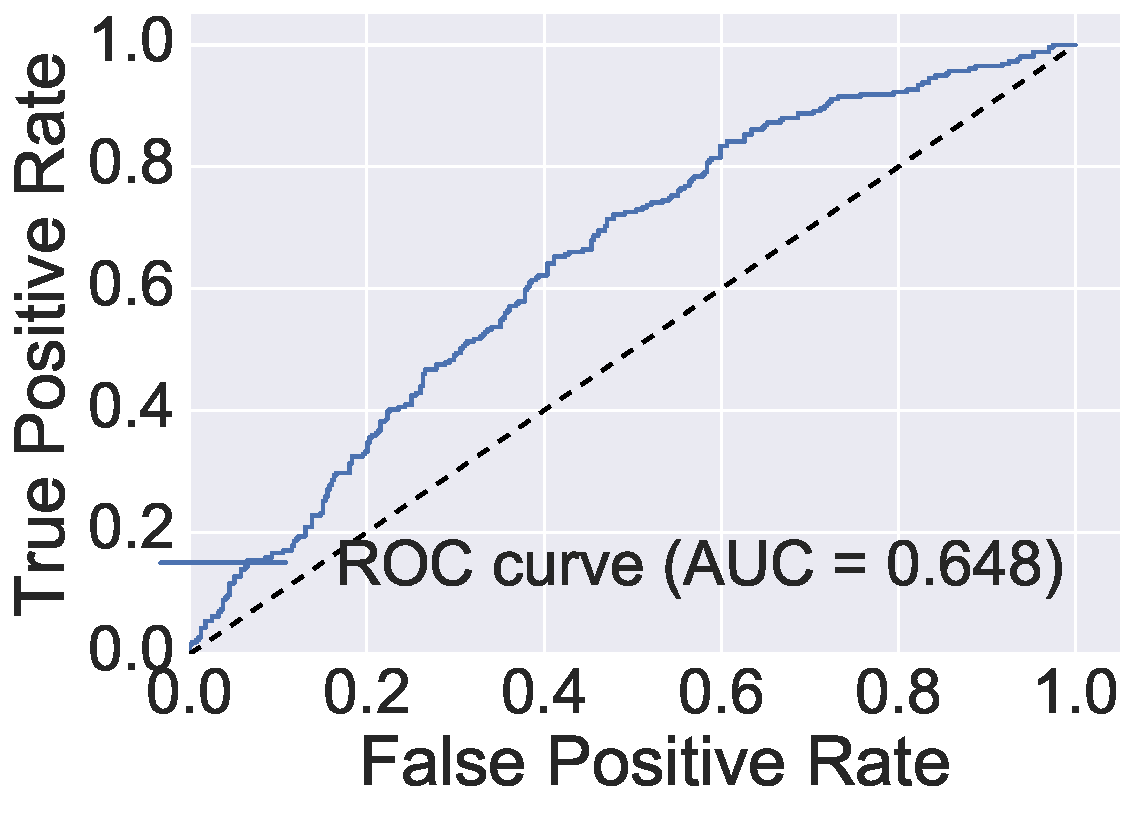
\includegraphics[width=.4\textwidth]{{/Users/ijoseph/Documents/Work/Graduate-Thesis/TeX/figures/ch4/cgp/mfaa_well_roc}.pdf}}%
  \qquad \\
  \subfloat[][Under-fit: $z_1 = 2, z_2 = 3$ .]{        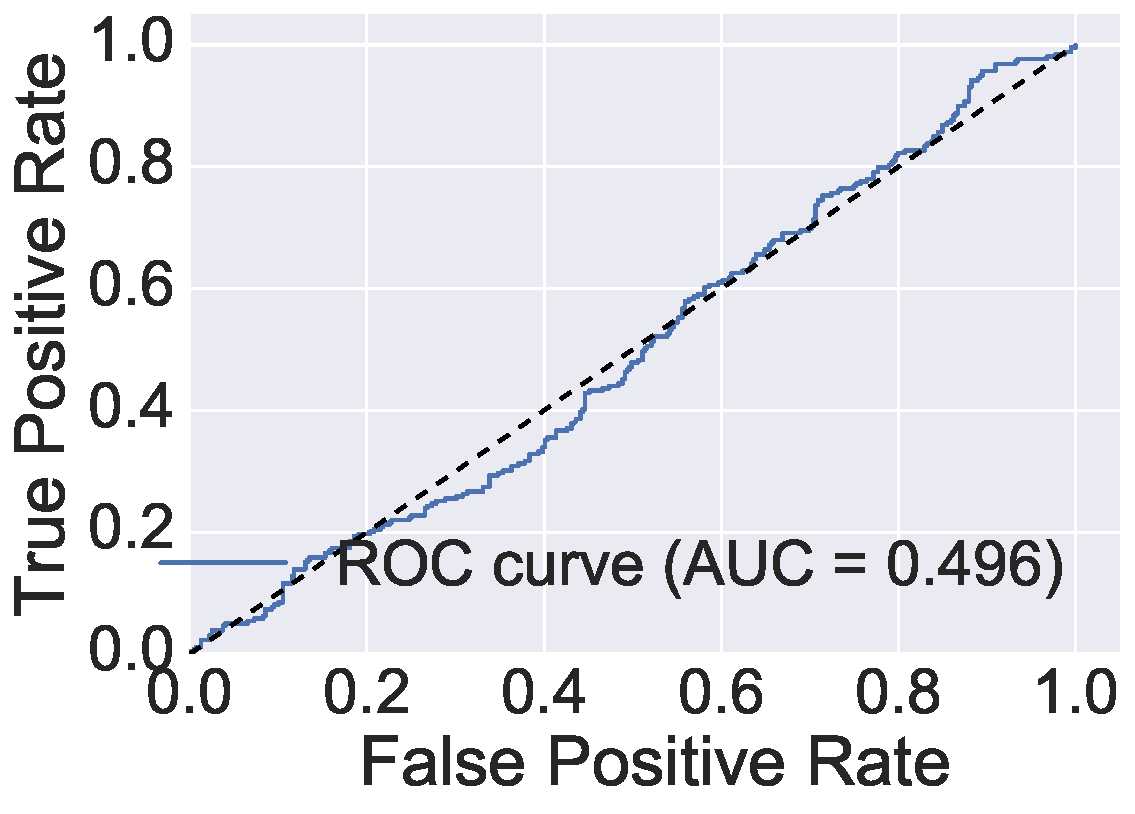
\includegraphics[width=.4\textwidth]{{/Users/ijoseph/Documents/Work/Graduate-Thesis/TeX/figures/ch4/cgp/mfaa_under_roc}.pdf}}%
  \qquad \\
\subfloat[][Closest to overfitting as possible: $z_1 = 62, z_2 =
65$. Note that the same AUC was the well-fit model was achieved at
this latent dimensionality. Higher latent dimensionality, which would
likely allow for AUC-degrading overfitting, was not possible as the
model currently is not implemented for latent dimensions higher than
the above.]{        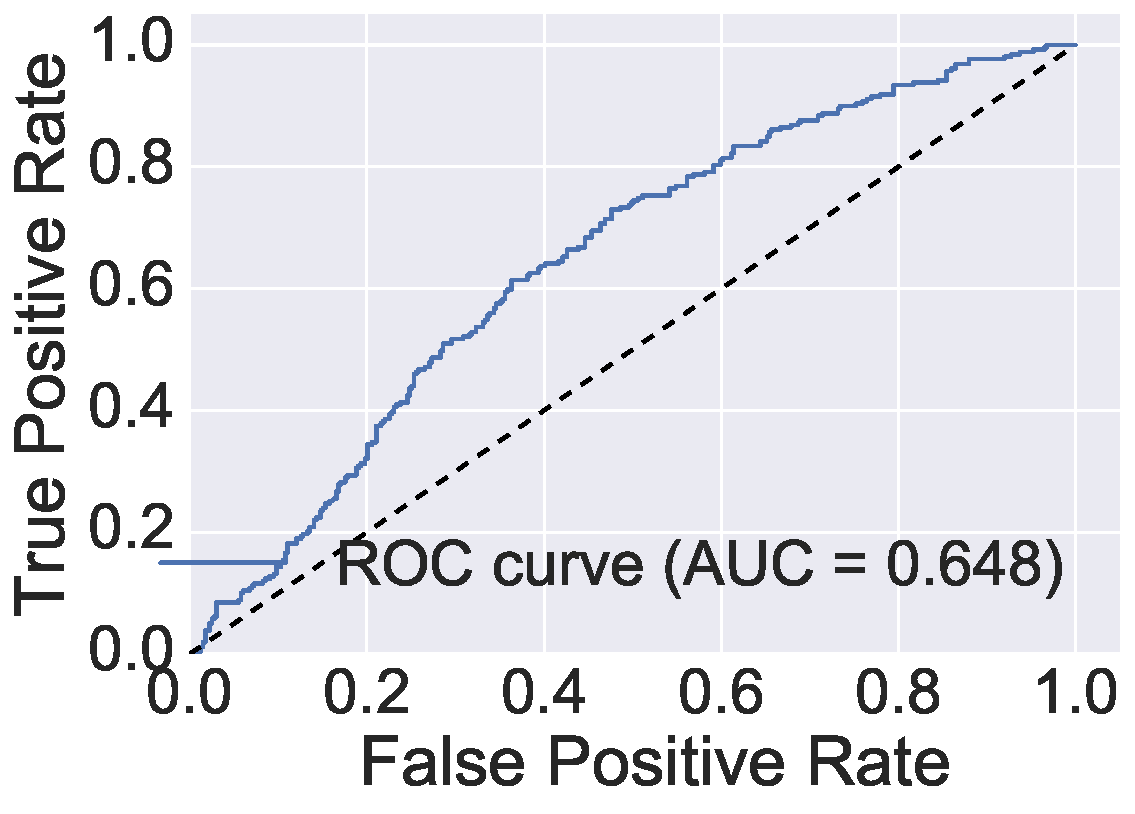
\includegraphics[width=.4\textwidth]{{/Users/ijoseph/Documents/Work/Graduate-Thesis/TeX/figures/ch4/cgp/mfaa_over_roc}.pdf}}%
  \caption{HFAM ROC curves for different levels of model
    complexity.} \label{fourcgpone}
\end{figure}
    

    \begin{figure} 
      \centering \subfloat[][Well-fit: $C = 1 \times 10^5$.]{\noindent
        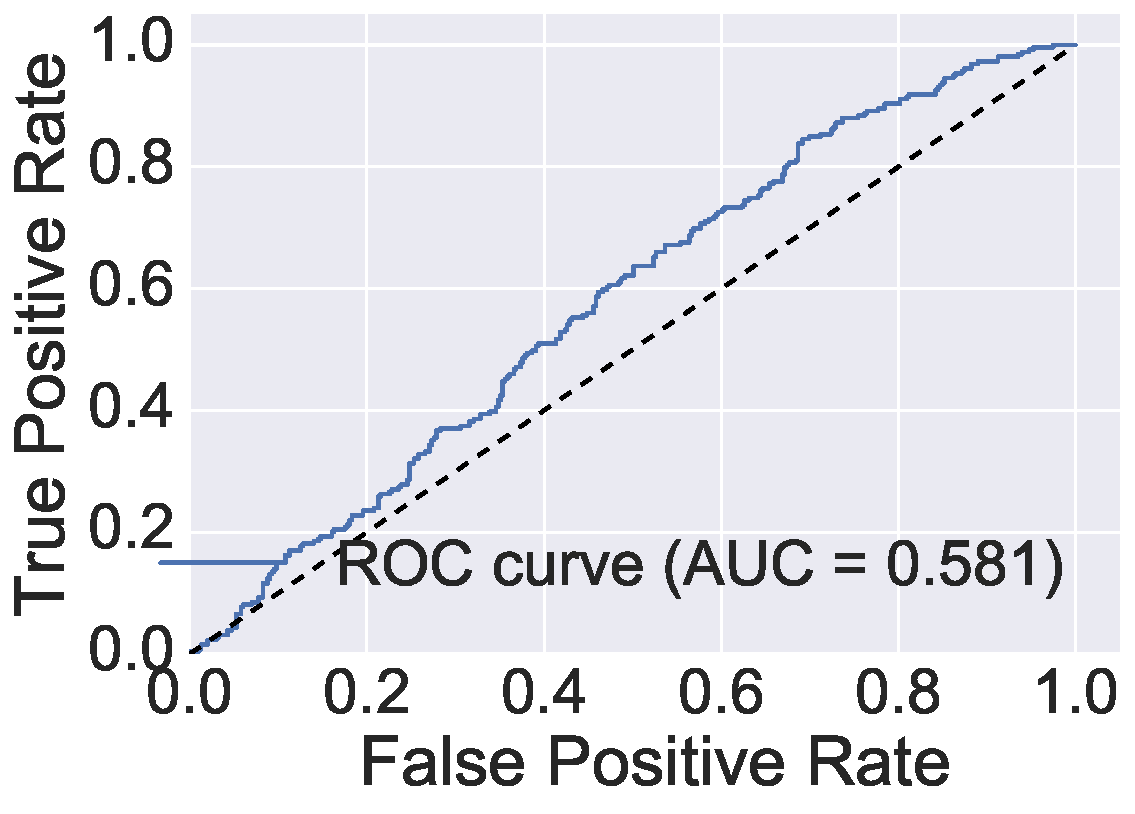
\includegraphics[width=.4\textwidth]{{/Users/ijoseph/Documents/Work/Graduate-Thesis/TeX/figures/ch4/cgp/log_reg_well_roc}.pdf}}%
      \qquad \\
      \subfloat[][Under-fit: $C = 1 \times 10^{-5}$
      .]{
        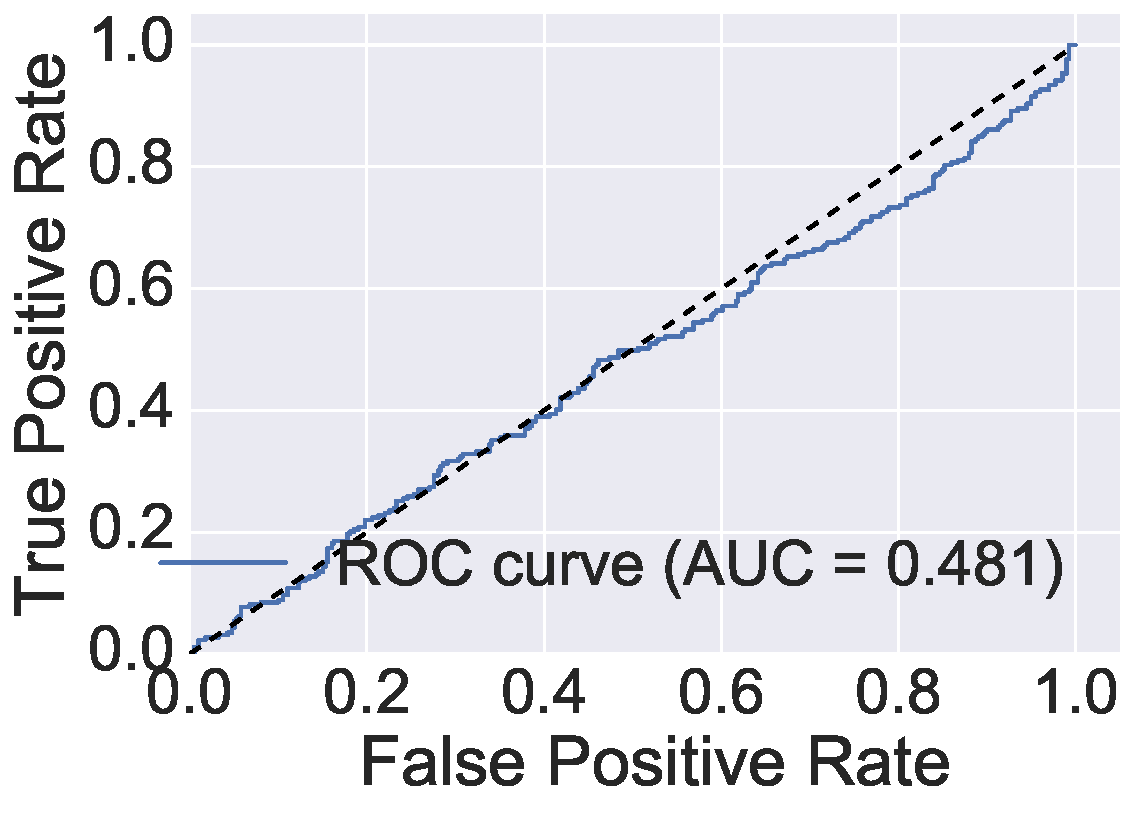
\includegraphics[width=.4\textwidth]{{/Users/ijoseph/Documents/Work/Graduate-Thesis/TeX/figures/ch4/cgp/log_reg_under_roc}.pdf}}%
      \qquad \\
      \subfloat[][Over-fit: $C = 1 \times 10^{15}$.]{
        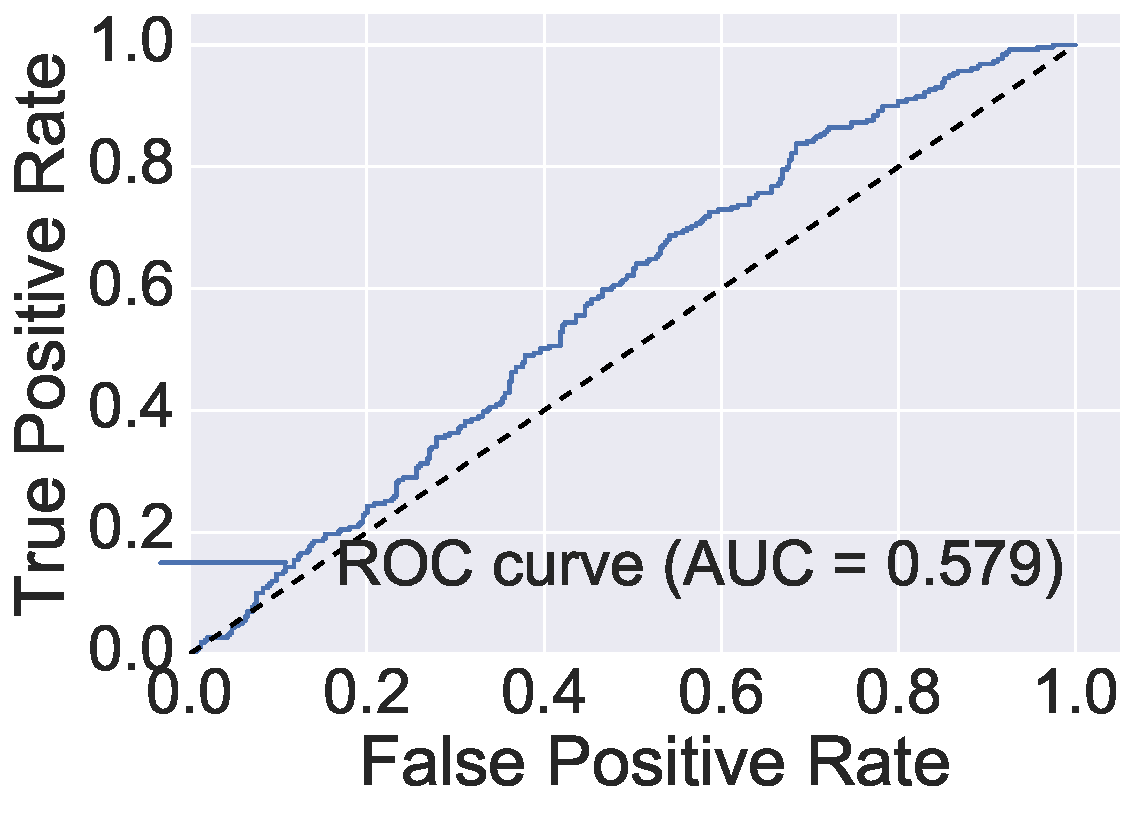
\includegraphics[width=.4\textwidth]{{/Users/ijoseph/Documents/Work/Graduate-Thesis/TeX/figures/ch4/cgp/log_reg_over_roc}.pdf}}%
      \caption{Logistic regression ROC curves for different levels of model
        complexity.} \label{fourcgptwo}
    \end{figure}

%% confusion

\begin{figure}
  \centering \subfloat[][Well-fit: $z_1 = 20, z_2 = 45$.]{\noindent
    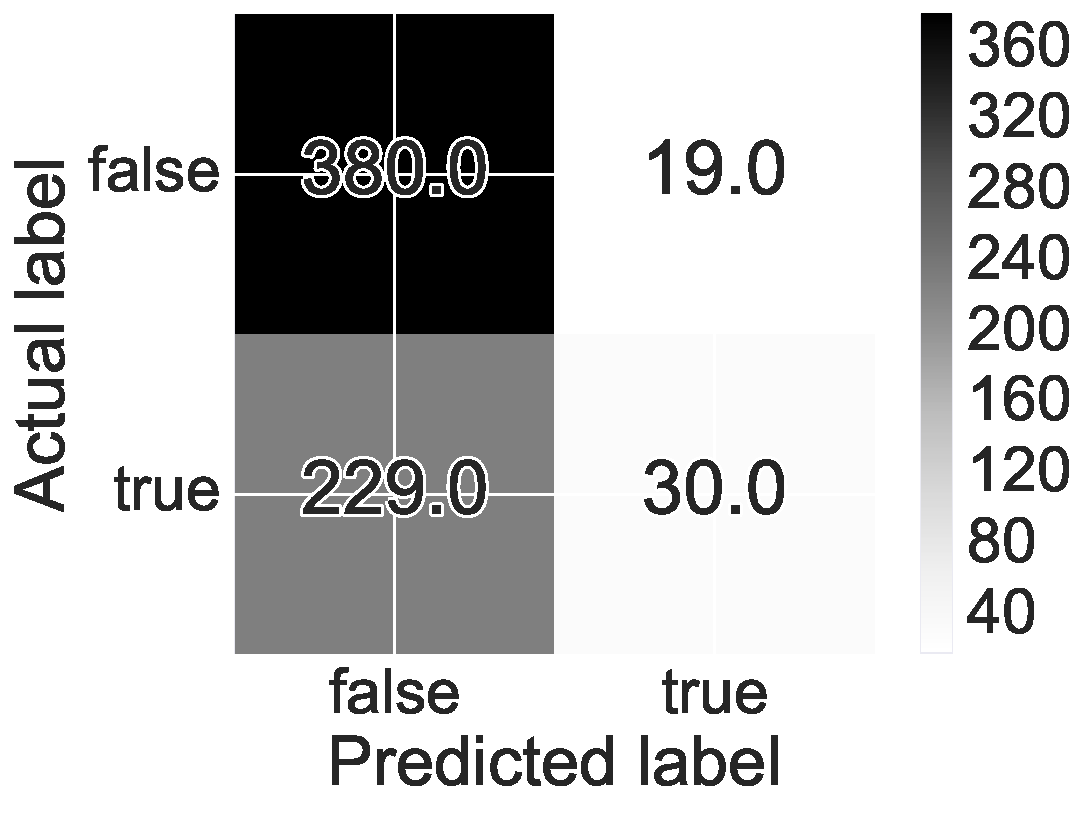
\includegraphics[width=.4\textwidth]{{/Users/ijoseph/Documents/Work/Graduate-Thesis/TeX/figures/ch4/cgp/mfaa_well_confus}.pdf}}%
  \qquad \\
  \subfloat[][Under-fit: $z_1 = 2, z_2 = 3$ .]{        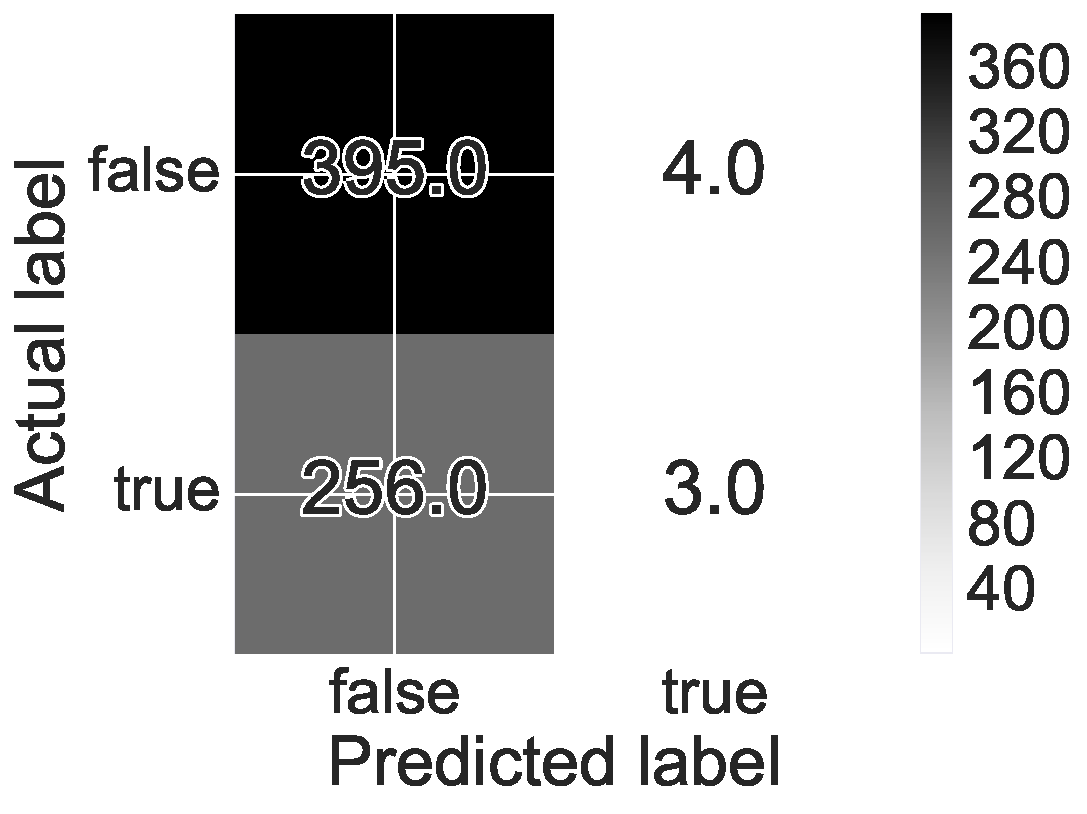
\includegraphics[width=.4\textwidth]{{/Users/ijoseph/Documents/Work/Graduate-Thesis/TeX/figures/ch4/cgp/mfaa_under_confus}.pdf}}%
  \qquad \\
  \subfloat[][Over-fit: $z_1 = 62, z_2 = 65$.]{        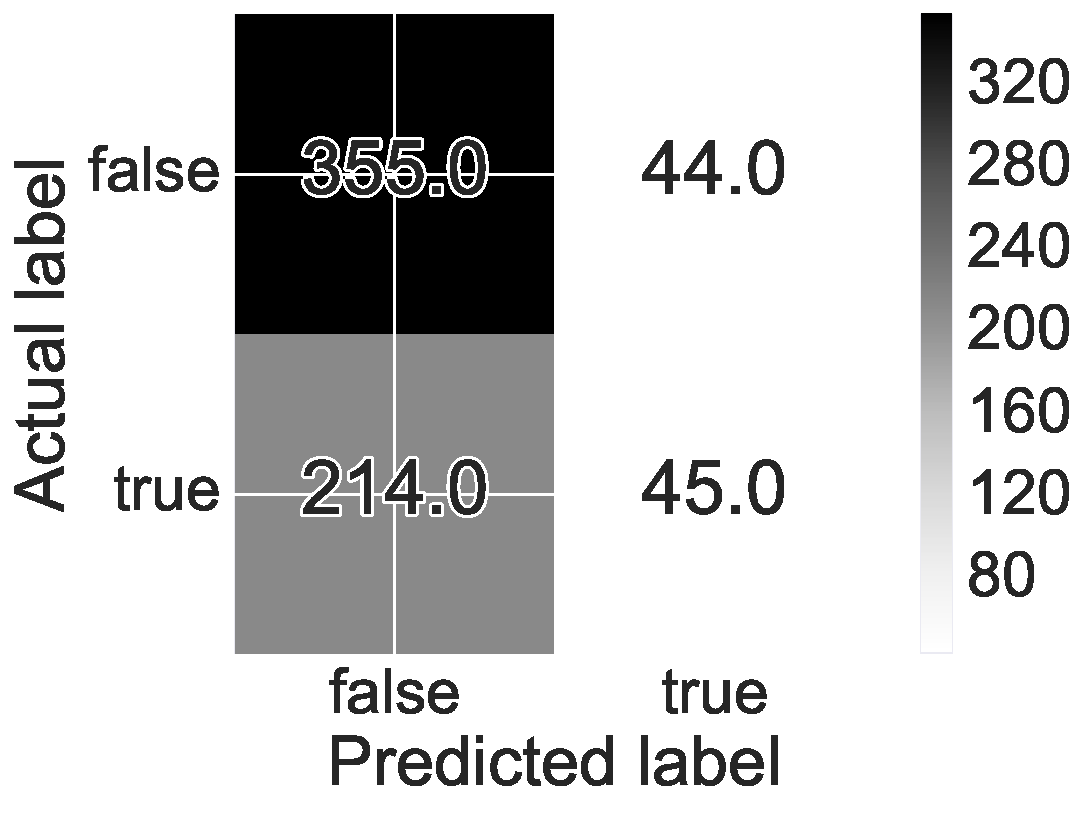
\includegraphics[width=.4\textwidth]{{/Users/ijoseph/Documents/Work/Graduate-Thesis/TeX/figures/ch4/cgp/mfaa_over_confus}.pdf}}%
  \caption{HFAM confusion matrices for different levels of model
    complexity.} \label{fourcgpthree}
\end{figure}
    

    \begin{figure} 
      \centering \subfloat[][Well-fit: $C = 1 \times 10^5$.]{\noindent
        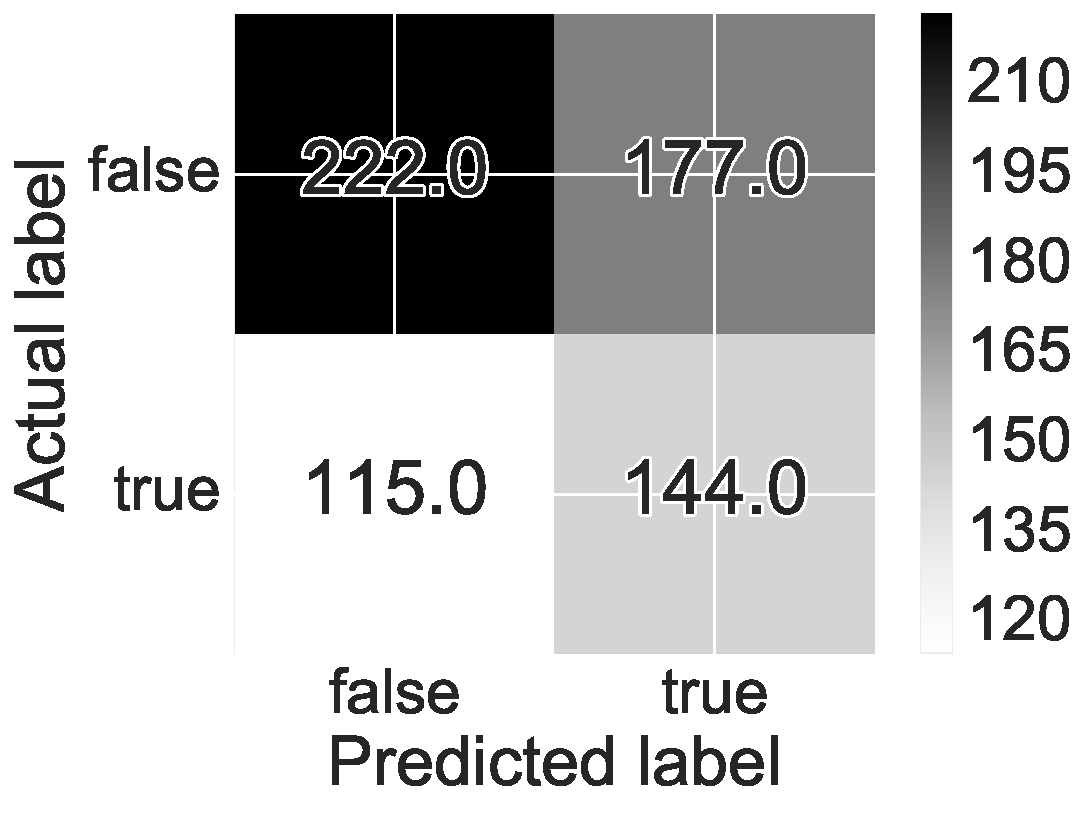
\includegraphics[width=.4\textwidth]{{/Users/ijoseph/Documents/Work/Graduate-Thesis/TeX/figures/ch4/cgp/log_reg_well_confus}.pdf}}%
      \qquad \\
      \subfloat[][Under-fit: $C = 1 \times 10^{-5}$
      .]{
        \includegraphics[width=.4\textwidth]{{/Users/ijoseph/Documents/Work/Graduate-Thesis/TeX/figures/ch4/cgp/log_reg_under_confus}.pdf}}%
      \qquad \\
      \subfloat[][Over-fit: $C = 1 \times 10^{15}$.]{
        \includegraphics[width=.4\textwidth]{{/Users/ijoseph/Documents/Work/Graduate-Thesis/TeX/figures/ch4/cgp/log_reg_over_confus}.pdf}}%
      \caption{Logistic regression confusion matrices for different levels of model
        complexity.} \label{fourcgpfour}
    \end{figure}

\subsection{Glioma outcome prediction}

The model's favorable performance is auspicious for its utility in the prediction of second-surgery hypermutation prediction using first-surgery sequencing data. However, time constraints and the relatively small number of samples available at the time of this writing preempted our ability to assess the model on combined datatypes. 

\begin{figure}
  \centering \includegraphics[width=.9\textwidth]{/Users/ijoseph/Documents/Work/Graduate-Thesis/TeX/figures/ch4/onedatatypecostello.pdf}
  \caption{Accuracy as assessed by
    $\frac{\text{true positives} + \text{true negatives} }{
      \text{false positives} + \text{false negatives}}$
    for two sequencing datatypes according to HFAM
    approximation. Results similar for logistic regression and linear
    discriminant analysis models.} \label{costelloresults}
\end{figure}


Assessment of single datatypes using existing methods, such as linear discriminant analysis and logistic regression, yielded that high AUC was not necessarily possible in this problem. We also assessed a non-probabilistic approximation of HFAM and found similarly inauspicious results (figure \ref{costelloresults}).. 

Thus, we might choose to use sequencing data collected post-second surgery to see if we could assess hypermutation as having already occurred (versus prediction of future hypermutation), as preliminary attempts to predict outcome from first-surgery tissue were unpromising. The utility of this would be the greater use of public datasets in order to assess the hypermutation phenotype when it is not explicitly accessible. 

We chose to use methylation and mutation information, as these datatypes were available for the highest number of samples.

In order to reduce dimensionality for the purposes of computational tractability and biologically mechanistic interpretability, we would choose the $50,000$ most variable methylation probes, pursuant to suggestions from Dr. Matthew Grimmer as to the most cogent way to reduce methylation dimensionality. In particular, this is hypothesized to be superior to alternate approaches. One possible alternate approach would be to binning based on specific regions, as related glioma methylation changes often occur on a single-CpG-site basis, rather than on a large scale basis.

\section{Discussion}

This approach shows promise; we feel that further refinement of the approach could yield to more accurate prediction than what is shown above. In particular, we would like to implement a model tuning phase above in order to assess dimensions; we would like to use the model to integrate more than two feature types -- a relatively simple addition on what is currently implemented. We would like to use different distributions for our observed datatypes that work more cogently with mutation information -- chiefly, the multinomial distribution.

We would like to assess the model versus existing non-probabilistic methods for heterogeneous, regularized supervised prediction as well, such as collaborative regression\cite{gross_collaborative_2015}. 

\chapter{Concluding statements}


\section{Conclusion}
Both methods described herein bring us closer to both of our goals: investigation and individualized treatment.

Both goals can be seen in a generalized learning framework, wherein either humans or machines develop and gather evidence towards models of molecular behavior that is inaccessible by direct, real-time observation.

For both human and machine learning, one needs to firstly identify low-level properties of a phenomenon; this can be seen as \textit{feature extraction} in the machine learning. One secondly needs to then use such low-level properties in order to form a coherent model of a phenomenon; this model could be described in words and be the result of several distinct perturbations of related as in the human case, or it could be pre-specified in form mathematically and features could be used as evidence in order to \textit{fit} a given mathematical model.

A classical example could be in vision, wherein spatial regions of light intensity and color correspond to features, and these are used to fit a model of possible structures in the world. The model fitting could be done in a human's brain based on pre-specified, empirically learned constraints on what physical object configurations are possible, or in computer vision by using a model pre-fit with such empirically-learned constraints. 

Here, we make progress on both regards, by (1) extracting the new features of fusion genes' expression and (2) creating a new model for fitting through abstract specification of how sequencing datatypes might correspond to an outcome of interest. 

\subsection{Feature extraction advances}

Features extracted from genomic data may be used individually by investigators with extensive knowledge of current cellular phenomena to generate more accurate causal models of various phenotypes, including oncogenesis, tumor progression, metastases, and survival. Here, we described the extraction of fusion genes' in a more accurate manner based on the use of expression information. The advance is thus twofold: (1) the addition of new features describing fusion gene expression where noen previously existed, and (2) more accurate presence of absence of intermediate features.

Specifically, the existence of RTK fusions in gliomas helped advance our knowledge of the centrality of such proteins in tumor progression within certain molecular classifications of LGG.
Our developed method allows for ease of doing so from future datasets. 

These features might also be included in a classifier consisting of a model to be fit, assessing survival time or progression.


\subsection{Automated modelling advances}

Models to be fit must accurately depict basic assumptions of the phenomenon or at least be robust to violations therein in order to be useful. Here, we successfully created a model that appears to be constitute useful baseline assumptions about how several sequencing datatypes available might relate to one another in ways meaningful for outcomes constituting the reactions to specific compounds.


\section{Outlook}

There is much further work to be done to further the use of genomic data for cancer investigation and individualized treatment. This work broadly involves possible advances in data collection, feature extraction, and models. 

\subsection{Data collection opportunities}

As evidence for a phenomenon increases with greater numbers of available observations, more observations would be of great use to increase evidence for relatively weak or rare yet important associations. More data would allow for models of higher complexity to be fit, which may more accurately represent the reality of tumor-related biological processes. It would also manifest in terms of more statistical significance for specific parameters related to increasing human understanding of these processes.

\subsubsection{Economic opportunities}

The cost of collecting genomic information from every patient still remains high in late 2016. In particular, whole genome sequencing (WGS) is typically infeasible for the majority of patients. WGS could be helpful to more accurately assess fusion gene existence and non-genic mutations and variants of interest. Sequencing with longer reads than around 100 base-pairs also remains problematically expensive, which limits our ability to resolve features related to fusion genes and repetitive regions of the genome in general. More detailed epigenetic data, such as histone modifications, could also be of use. 

This cost is particularly concerning due to it excluding the majority of humanity, which does not live in a so-called ``developed'' country able to fund such collection\cite{_97_2015}; even within ``developed'' countries, the majority of diagnosed cancer patients do not have access to facilities performing or organizing sequencing-based assessment. Even if access is possible, the high cost of sequencing (on the scale of $10^4$) not covered by insurance is prohibitive\cite{regalado_why_2016}. This concern is compounded by the fact that such populations also typically lack access to other medical resources and that such lack is arguably not a direct result of any inaction or action by individuals in these populations. Thus, much progress is possible in terms of collecting high amounts of sequencing information from a greater subset of the global population. 

\subsubsection{Data sharing opportunities}

Currently, accessing large amounts of high-quality, well-curated genomic tumor sequencing data is difficult. This is, according to this author, largely due to scientific incentive schemes which are developed around the idea of an individual investigator only directly using data that he or she collects in his or her individual facilities.

Such incentives manifest in the form of manuscript-based compensation assessments, wherein the vast minority of contributors receives the majority of credit. Individualistic incentives also manifest in the form of funding allotments which focus on individual researchers' goals and accomplishments. These incentives are inconsistent with the cost of sequencing and the ability to directly increase the utility of any specific scientific inquiry or model development through the use of others' data. Thus, much rethinking and adaptation of such incentives would be fruitful. 

Additionally, knowledge-sharing necessary for investigations that span disciplines such as this one is disincentivized in the above schemes and also due to an underemphasis on management ability. 

A small handful of institutions such as the Broad Institute, the Institute for Systems Biology, the Memorial Sloan-Kettering Cancer Center, and the Fred Hutchinson Cancer Research Center have made some progress in reframing the context in which tumor genomic data is assessed in order to address these issues by providing common funding for a segment of researchers and common incentive schemes across groups of researchers. Consortium efforts modeled after the Human Genome Project\cite{lander_initial_2001} such as TCGA also provide important progress in this area, but much room for improvement still remains. 

\subsection{Feature extraction opportunities}

There is room for improvement in terms of both the accuracy of current feature
assessment and in terms of the collection of new, potentially orthogonal sources of information.

\subsubsection{Opportunities for increased accuracy of current features}

All sequencing datatypes mentioned above could be more accurately converted into features than they are currently. 

Higher-depth and longer-read sequencing would provide more confident detection of specific mutations.  This would lead to improvement in the detection and assignment of fusion genes; some of this may come with an increased availability of more robust datatypes, such as sequencing that uses longer reads or higher depth. 

Gene expression features could be collected in a way that more closely relates to which proteins exist in or on the cell at a given point in time, as expressed RNA is merely a surrogate for this true parameter of interest. Ribosomal profiling\cite{ingolia_genome-wide_2009} and reverse-phase protein assay\cite{tibes_reverse_2006} are currently developing technologies for doing so, but limited information exists from these technologies as of this writing. 


\subsubsection{Additional feature opportunities}
New sequencing technologies will also be able to shed light on additional features of interest.

In addition to those mentioned above, more epigenetic information could be extracted, such as using as through the use of HI-C\cite{yaffe_probabilistic_2011} or histone mark-based assessment strategies.

\subsection{Model improvement opportunities}

There exists substantial room for improvement in terms of the specification of integrative models involving several different sequencing datatypes. As the availability of new and more features increases rapidly, model specification innovation needs to follow in order to adapt these new features most effectively towards the goals of investigation and individualized treatment. This will involve the study of these new features' behavior and their relationship to known biological mechanisms. 

One area of possible development that may become useful in this sphere is the use of non-linear models, which may more accurately reflect the behavior of enzymes outside of certain regions and other nonlinear biochemical processes. One promising way that this may be accomplished is through the use of multilayer neural networks models, which can be viewed as automatically extracting higher-level features via nonlinear combinations of existing features \cite{jesse_dunietz_fundamental_2016}.
\sloppy
\printbibliography
\begin{appendices}
  \chapter{Three-node model formulation}
\section{Model}
\begin{center}
\includegraphics[width=\textwidth/3]{MFAA.png}
\end{center}
\newcommand{\fulljointp}{P \left(
  \{\x_{i,n}\}_{i=1}^3,\{ \z_{j,n}\}_{j=1}^2| \{\W_k\}_{k=0}^3,
    \{\bpsi_{\ell}\}_{\ell=0}^3 \right)}
\begin{align*}
  \fulljointp &= P(\z_1) P(\z_2 | \z_1) P(\x_1 | \z_2) P(\x_2 | \z_2)
                P(\x_3 | \z_1) \\
  \z_1 &\sim N(\vec{0}, \I ) \inreala{m}{1} \\
  \z_2| \z_1 &\sim N(\W_0 \z_1, \bpsi_0) \inreala{p_0}{1}\\
  \x_1 | \z_2 &\sim N(\W_1 \z_2, \bpsi_1) \inreala{ p_1}{1}\\
  \x_2 | \z_2 &\sim N(\W_2 \z_2, \bpsi_2) \inreala{p_2}{1} \\
  \x_3 | \z_1 &\sim N(\W_3 \z_1, \bpsi_3) \inreala{p_3}{1}
\end{align*}
%This implies the following dimensions for parameters $\W$ and $\bpsi$:
\begin{align*}
  \W_0 &\inreala{p_0}{m} &   \bpsi_0 &\inreala{p_0}{p_0} \\
  \W_1 &\inreala{p_1}{p_0} &  \bpsi_1 &\inreala{p_1}{p_1}\\
  \W_2 &\inreala{p_2}{p_0} &   \bpsi_2 &\inreala{p_2}{p_2}\\
  \W_3 &\inreala{p_3}{m} &         \bpsi_3 &\inreala{p_3}{p_3}\\  
\end{align*}

\begin{landscape}
\section{Complete log-likelihood}
For $N$ samples, 
\begin{equation}
\begin{split}
\ell_n(\Theta) \coloneqq \sum_{n=1}^N & \log  \left( \fulljointp \right) = \\
&\sum_{n=1}^N -\frac{p_1}{2} \log (2 \pi) - \frac{1}{2} \log(|\bpsi_1|) -
\frac{1}{2} \left( \left( \x_{1,n} - \W_1 \z_{2,n} \right)^T \bpsi_1^{-1} \left(
    \x_{1,n} - \W_1 \z_{2,n} \right) \right) + \\
& -\frac{p_2}{2} \log (2 \pi) - \frac{1}{2} \log(|\bpsi_2|) -
\frac{1}{2} \left( \left( \x_{2,n} - \W_2 \z_{2,n} \right)^T \bpsi_2^{-1} \left(
    \x_{2,n} - \W_2 \z_{2,n} \right) \right) + \\
& -\frac{p_3}{2} \log (2 \pi) - \frac{1}{2} \log(|\bpsi_3|) -
\frac{1}{2} \left( \left( x_{3,n} - \W_3 \z_{1,n} \right)^T \bpsi_3^{-1} \left(
    \x_{3,n} - \W_3 \z_{1,n} \right) \right) + \\
& -\frac{p_0}{2} \log (2 \pi) - \frac{1}{2} \log(|\bpsi_0|) -
\frac{1}{2} \left( \left( \z_{2,n} - \W_0 \z_{1,n} \right)^T \bpsi_0^{-1} \left(
    \z_{2,n} - \W_0 \z_{1,n} \right) \right) + \\
& -\frac{m}{2} \log (2 \pi) - \frac{1}{2} \z_{1,n}^T \z_{1,n} 
\end{split}
\end{equation}



\newcommand{\ecll}{\ev_{\{ \z_j\}_{j=1}^2 | \{\x_i\}_{i=1}^3}
  \left[ \sum_{n=1}^N \log \left( \fulljointp \right) \right] }
\begin{equation}
\begin{split}
\Rightarrow & \ecll= \\
& \sum_{n=1}^N - \frac{p_1}{2} \log (2\pi) - \frac{1}{2} \log( |\bpsi_1| ) -
\frac{1}{2} \left(
  \x_{1,n}^T \bpsi_1^{-1} \x_{1,n} - 2 \x_{1,n}^T    \bpsi_1^{-1} \W_1 \ev[ \z_{2,n}] +
  \Tr \left( \ev[\z_{2,n} \z_{2,n}^T ] \W_1^T  \bpsi_1^{-1}
    \W_1\right) \right)\\
& - \frac{p_2}{2} \log (2\pi) - \frac{1}{2} \log( |\bpsi_2| ) -
\frac{1}{2} \left(
\x_{2,n}^T \bpsi_2^{-1} \x_{2,n} - 2 \x_{2,n}^T    \bpsi_2^{-1} \W_2 \ev[\z_{2,n}] +
  \Tr \left( \ev[\z_{2,n} \z_{2,n}^T ] \W_2^T  \bpsi_2^{-1}
    \W_2\right) \right)\\
& - \frac{p_3}{2} \log (2\pi) - \frac{1}{2} \log( |\bpsi_3| ) -
\frac{1}{2} \left(
\x_{3,n}^T \bpsi_3^{-1} \x_{3,n} - 2 \x_{3,n}^T    \bpsi_3^{-1} \W_3 \ev[\z_{1,n} ]+
  \Tr \left( \ev[\z_{1,n} \z_{1,n}^T ] \W_3^T  \bpsi_3^{-1}
    \W_3\right) \right)\\
& - \frac{p_0}{2} \log (2\pi) - \frac{1}{2} \log( |\bpsi_0| ) -
\frac{1}{2} \left(
\Tr \left( \ev [\z_{2,n} \z_{2,n}^T] \bpsi_0^{-1} \right)  - 2 \Tr \left( \ev[\z_{1,n}\z_{2,n}^T]
  \bpsi_0^{-1} \W_0 \right) +
  \Tr \left( \ev[\z_{1,n} \z_{1,n}^T ] \W_0^T  \bpsi_0^{-1}
    \W_0\right) \right)\\
& -\frac{m}{2} \log( 2 \pi) - \frac{1}{2} \ev [ \z_{1,n}^T \z_{1,n}]
\end{split}
\end{equation}
\end{landscape}
\pagebreak
\section{M-Step: finding critical points}
\subsection{$\W$}

% W_0
\begin{align*}
  &\frac{  \partial }{\partial \W_0} \ecll \\
  &=  \sum_{n=1}^N \frac{\partial}{\partial \W_0} \Tr \left(\ev [\z_{1,n} \z_{2,n}^T]
      \bpsi_0^{-1} \W_0 \right) - \frac{1}{2} \frac{\partial}{\partial
      \W_0 }\Tr \left( \ev [ \z_{1,n}
    \z_{1,n}^T] \W_0^T \bpsi_0^{-1} \W_0 \right) \\
  &=  \ev [\z_{1,n} \z_{2,n}^T] \bpsi_0^{-1} - \ev [\z_{1,n} \z_{1,n}^T] \W_0^T
    \bpsi_0^{-1}\\
   \Rightarrow \Aboxed{ \hat{\W_0^T}_{\text{MLE}} &= \left(
                                                    \sum_{n=1}^N \ev [\z_{1,n} \z_{1,n}^T]
      \right)^{-1} \left( \sum_{n=1}^N \ev [\z_{1,n} \z_{2,n}^T] \right)}\\
\end{align*}

\begin{align*}
  &\frac{\partial} {\partial \W_1} \ecll \\
  &= \sum_{n=1}^N \frac{\partial}{\partial \W_1} \x_{1,n}^T \bpsi_1^{-1} \W_1 \ev
    [\z_{2,n}] - \frac{1}{2} \frac{\partial}{\partial \W_1} \Tr \left( \ev
    [\z_{2,n} \z_{2,n}^T] \W_1^T \bpsi_1^{-1} \W_1 \right)\\
  &= \ev[\z_{2,n}] \x_{1,n}^T \bpsi_1^{-1} - \ev [ \z_{2,n} \z_{2,n}^T] \W_1^T
    \bpsi_1^{-1} \\
    \Rightarrow \Aboxed{ \hat{ \W_1^T }_{\text{MLE}} &= \left(
                                                       \sum_{n=1}^N
                                                       \ev [ \z_{2,n}
                                                       \z_{2,n}^T]
                                                       \right)^{-1}
                                                       \left(
                                                       \sum_{n=1}^N \ev [ \z_{2,n}]
      \x_{1,n}^T  \right)}
\end{align*}

By pattern-matching,
\begin{align*}
\Aboxed{  \hat{\W_2^T}_{\text{MLE}} &= \left( \sum_{n=1}^N \ev [ \z_{2,n} \z_{2,n}^T] \right)^{-1}
                              \left( \sum_{n=1}^N \ev [ \z_{2,n}]
                                      \x_{2,n}^T  \right)}\\
\Aboxed{    \hat{\W_3^T}_{\text{MLE}} &= \left( \sum_{n=1}^N \ev [ \z_{1,n} \z_{1,n}^T] \right)^{-1}
                              \left( \sum_{n=1}^N \ev [ \z_{1,n}] \x_{3,n}^T \right)}\\  
\end{align*}
\pagebreak
\begin{landscape}
\subsection{$\bpsi$}


\begin{align*}
  &\frac{\partial}{\partial \bpsi_0} \ecll = \\
  & \sum_{n=1}^N \left( - \frac{\partial}{\partial \bpsi_0}  \frac{1}{2} \log \left( \left|
    \bpsi_0 \right| \right) - \frac{1}{2} \frac{\partial}{\partial
    \bpsi_0}\Tr \left( \ev [\z_{2,n} \z_{2,n}^T] \bpsi_0^{-1} \right)
    + \\
    &\frac{\partial}{\partial \bpsi_0} \Tr \left( \ev [\z_{1,n} \z_{2,n}^T ]
    \bpsi_0^{-1} \W_0 \right) - \frac{1}{2} \frac{\partial}{\partial \bpsi_0} \Tr
    \left( \ev [\z_{1,n} \z_{1,n}^T] \W_0^T \bpsi_0^{-1} \W_0 \right) \right) \\
    &=\sum_{n=1}^N \left( -\frac{1}{2} \bpsi_0^{-1}  + \frac{1}{2} \bpsi_0^{-1} \ev[\z_{2,n} \z_{2,n}^T] \bpsi_0^{-1} - \bpsi_0^{-1} \ev[\z_{2,n} \z_{1,n}^T] \W_0^T
      \bpsi_0^{-1} + \frac{1}{2} \bpsi_0^{-1} \W_0 \ev [\z_{1,n} \z_{1,n}^T ] \W_0^T
      \bpsi_0^{-1}\right) \\
  \Rightarrow \hat{\bpsi_0}_{\text{MLE}} &= \frac{1}{N}  \sum_{n=1}^N \left( \ev[ \z_{2,n} \z_{2,n}^T] - 2 \ev [\z_{2,n} \z_{1,n}^T] \W_0^T +  \W_0 \ev[\z_{1,n}
    \z_{1,n}^T] \W_0^T       \right)
\end{align*}
By pattern-matching, 
\begin{align*}
 \hat{\bpsi_1}_{\text{MLE}} &=  \frac{1}{N}  \sum_{n=1}^N \left( \x_{1,n} \x_{1,n}^T - 2 \x_{1,n}
                                        \ev[\z_{2,n}^T] \W_1^T +  \W_1 \ev[\z_{2,n}
                                \z_{2,n}^T] \W_1^T      \right) \\
 \hat{\bpsi_2}_{\text{MLE}} &= \frac{1}{N}  \sum_{n=1}^N \left( \x_{2,n} \x_{2,n}^T - 2 \x_{2,n}
                                           \ev[\z_{2,n}^T] \W_2^T +  \W_2 \ev[\z_{2,n}
                                  \z_{2,n}^T] \W_2^T       \right) \\
 \hat{\bpsi_3}_{\text{MLE}} &=  \frac{1}{N}  \sum_{n=1}^N \left( \x_{3,n} \x_{3,n}^T - 2 \x_{3,n} \ev[\z_{1,n}^T] \W_3^T + \W_3 \ev[\z_{1,n}
    \z_{1,n}^T] \W_3^T      \right) \\
\end{align*}

Using a generalized EM algorithm, and therefore substituting $\W$ with
$\hat{\W}_{\text{MLE}}$ in $\hat{\bpsi}_{\text{MLE}}$:

\begin{align*}
\Aboxed{ \hat{\bpsi_0}_{\text{MLE}} &=  \frac{1}{N}  \sum_{n=1}^N \left( \ev[\z_{2,n} \z_{2,n}^T] -  \ev [\z_{2,n} \z_{1,n}^T]
                             \left( \ev [z_{1,n} \z_{1,n}^T ] \right)^{-1} \ev[
                                      \z_{1,n} \z_{2,n}^T] \right) }\\
\Aboxed{   \hat{\bpsi_1}_{\text{MLE}} &=\frac{1}{N}  \sum_{n=1}^N  \left( \x_{1,n} \x_{1,n}^T - \x_{1,n} \ev[\z_{2,n}^T]
                                        \left( \ev [\z_{2,n} \z_{2,n}^T
                                        ]\right)^{-1} \ev[\z_{2,n}]
                               \x_{1,n}^T \right)}\\
  \Aboxed{   \hat{\bpsi_2}_{\text{MLE}} &= \frac{1}{N}  \sum_{n=1}^N  \left( \x_{2,n} \x_{2,n}^T - \x_{2,n} \ev[\z_{2,n}^T]
                                        \left( \ev [\z_{2,n} \z_{2,n}^T
                                        ]\right)^{-1} \ev[\z_{2,n}]
                                 \x_{2,n}^T \right)}\\
    \Aboxed{   \hat{\bpsi_3}_{\text{MLE}} &= \frac{1}{N}  \sum_{n=1}^N
                                            \left( \x_{3,n} \x_{3,n}^T - \x_{3,n} \ev[\z_{1,n}^T]
                                        \left( \ev [\z_{1,n} \z_{1,n}^T
                                        ]\right)^{-1} \ev[\z_{1,n}] \x_{3,n}^T
                                            \right)}\\
\end{align*}

Note that in the case of assuming diagonal errors $\bpsi_i$, we simply
take the diagonal component of every $\bpsi_i$ when performing each
update. 

\begin{align}
  \hat{\bpsi}_{i, \text{MLE}} \coloneqq \text{diag}
  \left(\hat{\bpsi}_{i, \text{MLE}} \right)
\end{align}
\pagebreak
\section{E-Step: finding posterior conditional distribution}


\newcommand{\zonezone}{\W_3^T \bpsi_3^{-1}\W_3 + \W_0^T\bpsi_0^{-1}\W_0+\I}
\newcommand{\zoneztwoT}{-\bpsi_0^{-1}\W_0}
\newcommand{\zoneztwo}{-\W_0^T \bpsi_0^{-1}}
\newcommand{\zonexthreeT}{-\bpsi_3^{-1}\W_3}
\newcommand{\zonexthree}{-\W_3^T \bpsi_3^{-1}}
\newcommand{\ztwoztwo}{\W_1^T \bpsi^{-1}_1 \W_1 + \W_2^T \bpsi^{-1}_2
  \W_2 + \bpsi_0^{-1}}
\newcommand{\ztwoxoneT}{-\bpsi_1^{-1}\W_1}
\newcommand{\ztwoxone}{-\W_1^T\bpsi_1^{-1}}
\newcommand{\ztwoxtwoT}{-\bpsi_2^{-1}\W_2}
\newcommand{\ztwoxtwo}{-\W_2^T \bpsi_2^{-1}}
\newcommand{\xonexone}{\bpsi_1^{-1}}
\newcommand{\xtwoxtwo}{\bpsi_2^{-1}}
\newcommand{\xthreexthree}{\bpsi_3^{-1}}
By inspection, 
\begin{align}
  \z_1, \z_2, \x_1, \x_2, \x_3 \sim N(\vmu, \bSigma), \text{where}
  \nonumber \\
  \bLambda \coloneqq \bSigma^{-1} =  \nonumber \\
  \begin{blockarray}{ccc|ccc}
    \ & \z_1 & \z_2 & \x_1 & \x_2 & \x_3 \\
    \begin{block}{c(cc|ccc)}
      \z_1 & \zonezone & \zoneztwo & \bold{0} & \bold{0} & \zonexthree  \\
      \z_2 & \zoneztwoT & \ztwoztwo & \ztwoxone & \ztwoxtwo & \bold{0}  \\ \cline{1-6}
      \x_1 & \bold{0} & \ztwoxoneT & \xonexone & \bold{0} & \bold{0}  \\
      \x_2 & \bold{0} & \ztwoxtwoT & \bold{0} & \xtwoxtwo & \bold{0} \\
      \x_3 & \zonexthreeT & \bold{0} & \bold{0} & \bold{0} & \xthreexthree \\
    \end{block}
  \end{blockarray} \label{joint.precision}\\ 
  \coloneqq
  \left(
  \begin{array}{c|c}
      \bLambda_{zz} & \bLambda_{zx} \\ \hline
      \bLambda_{xz} & \bLambda_{xx} \\
  \end{array}
  \right) \nonumber \\
\text{, where } \x \coloneqq \colvec{3}{\x_1}{\x_2}{\x_3}, \z
  \coloneqq \colvec{2}{\z_1}{\z_2} \label{x.and.z.vector.def}
\end{align}
\end{landscape}
\pagebreak

\subsection{Working with precision matrix}

% define bLambdas
\newcommand{\lambdazz}{\begin{pmatrix} \zonezone & \zoneztwo \\
      \zoneztwoT & \ztwoztwo \end{pmatrix}}

\newcommand{\lambdazx}{\begin{pmatrix} \mathbf{0} & \mathbf{0} & \zonexthree \\
    \ztwoxone & \ztwoxtwo & \bold{0} \end{pmatrix}}

\newcommand{\lambdaxz}{\begin{pmatrix} \mathbf{0} & \ztwoxoneT \\
    \mathbf{0} & \ztwoxtwoT \\
    \zonexthreeT & \mathbf{0} \\
  \end{pmatrix}}

\newcommand{\lambdaxx}{\begin{pmatrix} \bpsi_1^{-1} & \mathbf{0} & \mathbf{0} \\
    \mathbf{0} & \bpsi_2^{-1} & \mathbf{0} \\
    \mathbf{0} & \mathbf{0} & \bpsi_3^{-1} \\
  \end{pmatrix}}



We know that
\begin{align}
  \z | \x &\sim N(\vmu_{z|x}, \bSigma_{z|x}) \text{ ,where} \\
  \vmu_{z|x} &= \vmu_{z} - \bLambda_{zz}^{-1} \bLambda_{zx} \left( \x -
               \vmu_x \right) \\
  \bSigma_{z|x} &= \bLambda_{zz}^{-1} \coloneqq    \left(
  \begin{array}{c|c}
      \bSigma_{z_1z_1|x} & \bSigma_{z_1z_2|x} \\ \hline
      \bSigma_{z_2z_1|x} & \bSigma_{z_2z_2|x} \\
  \end{array}
  \right) 
\end{align}



\subsubsection{Finding $\vmu_{z|x}$ by expanding $(5)$}

\begin{align}
  \vmu &= \vec{0}^{d \times 1}\text{, where }  d \coloneqq m +
         \sum_{i=0}^3 p_i \\
         \vmu &\coloneqq \colvec{2}{\vmu_z}{\vmu_x} \text{ , where }
                \vmu_z \inreala{\left(m + p_0\right)}{1}, \vmu_x \inreala{\left(p_1
                + p_2 + p_3 \right)}{1} \nonumber \\
                \Rightarrow \vmu_{z|x} &= - \bLambda_{zz}^{-1}
  \bLambda_{zx} \x
\end{align}
Now we have what we need for the E-step:

\begin{align}
 \Aboxed{ \ev[\z_1| \x] &=  \vmu_{z_1 |x} } \label{postexp:1} \\
\Aboxed{  \ev[\z_2| \x] &=  \vmu_{z_2 |x} }\\
\Aboxed{  \ev[\z_1\z_1^T | \x] &= \bSigma_{z_1z_1|x} +
                         \vmu_{z_1|x}\vmu_{z_1|x}^T}\\
\Aboxed{    \ev[\z_2\z_2^T | \x] &= \bSigma_{z_2z_2|x} +
                           \vmu_{z_2|x}\vmu_{z_2|x}^T }\\
\Aboxed{      \ev[\z_1\z_2^T | \x] &= \bSigma_{z_1z_2|x} + \vmu_{z_1|x}\vmu_{z_2|x}^T                }\label{postexp:5}
\end{align}


\pagebreak % fail
\section{Finding conditional distribution of outcome observed variable
  given input observed variables}
For the purposes of classification, we observe $\x_1$ and $\x_2$ and
would like to predict $\x_3$ based on parameters learned during
fitting on training data $\hat{\bTheta} \coloneqq \left\{ \{\hat{W}_k\}_{k=0}^3 ,
  \{\hat{\bpsi}_\ell\}_{\ell=0}^3  \right\}$. Thus, we're interested in
obtaining an expression for:
\begin{align}
\ev [ \x_3 | \x_1, \x_2, \bTheta]
\end{align}

We obtain this first based on partitioning the joint covariance matrix and
partitioned Gaussian identities (\ref{partitioning}), and then based on the direct integral form of the expectation (\ref{direct}).
\subsection{Partitioning} \label{partitioning}
By equation \ref{joint.precision} and by partitioning, 
\begin{align}
  \bSigma &=  \bLambda^{-1} \\
&= \left(
  \begin{array}{c|c}
      \bSigma_{zz} & \bSigma_{zx} \\ \hline
      \bSigma_{xz} & \bSigma_{xx} \\
  \end{array}
  \right) 
\end{align}, where $\x$ and $\z$ are defined as in \ref{x.and.z.vector.def}.


Since the marginal distribution of a partition of a Gaussian has
the joint covariance of that same partition, the joint distribution
of the observed variables will have covariance $\bSigma_{xx}$. 


We can then obtain the marginal observed precision matrix
($\bLambda'$) by inverting, can expand this into
blocks for each observed variable, and partition between observed and
prediction variables:

\begin{align}
  \bLambda' &\coloneqq \bSigma_{xx}^{-1} \\
  &= \left(
  \begin{array}{cc|c}
      \bLambda'_{x_1x_1} & \bLambda'_{x_1x_2} & \bLambda'_{x_1x_3} \\
      \bLambda'_{x_2x_1} & \bLambda'_{x_2x_2} & \bLambda'_{x_2x_3} \\
    \hline
      \bLambda'_{x_3x_1} & \bLambda'_{x_3x_2} & \bLambda'_{x_3x_3} \\
  \end{array}
  \right) 
\end{align}

By partitioned Guassian identity (2.97 of Bishop's \textit{Pattern Recognition and Machine
  Learning}), $\x_3| \x_1, \x_2$ is distributed as a Gaussian with expectation:

\begin{align}
  \ev [ \x_3 | \x_1, \x_2, \bTheta]   &=  \vmu_{x_3} - \left(
                                        \bLambda'_{x_3 x_3}
                                        \right)^{-1} \left(\begin{array}{cc}
                                                       \bLambda'_{x_3x_1}
                                                       &
                                                         \bLambda'_{x_3x_2}                                                    
\end{array} \right)  \left( \colvec{2}{\x_1}{\x_2} -
  \colvec{2}{\vmu_{x_1}} {\vmu_{x_2}} \right) \\
\end{align}, where $\vmu_{x_i}$ are additional parameters learned
during fitting step. 

\subsection{Direct} \label{direct}

Starting with the general form for conditional expectation,

\begin{align}
    \ev_\bTheta \left[ \x_3 | \x_1, \x_2 \right] &= \int \x_3 P(\x_3 | \x_1, \x_2) d\x_3 \\
    &= \int \x_3 \frac{P(\x_1, \x_2, \x_3)}{P(\x_1, \x_2)} d\x_3 \\
    &= \int \int \int \x_3 \frac{ P(\x_1, \x_2, \x_3 , \z_1, \z_2) }{P(\x_1, \x_2)} d \z_1 d\z_2 d\x_3 \\ 
    &= \int \int \int \x_3 \frac{ P(\x_1, \x_2, \x_3 , \z_1, \z_2) }{P(\x_1, \x_2)} d \x_3 d\z_1 d\z_2 \\ 
    &= \int \int \frac{P(\x_1, \x_2, \z_1, \z_2)}{P(\x_1, \x_2)} \left( \int \x_3 P(\x_3 | \z_1) d \x_3 \right) d\z_1 d\z_2 \label{line.27} \\ 
    &= \int \int \frac{P(\x_1, \x_2, \z_1, \z_2)}{P(\x_1, \x_2)} \left( \ev_\bTheta \left[ \x_3 | \z_1 \right] \right) d\z_1 d\z_2 \\ 
    &= \int \int \frac{P(\x_1, \x_2, \z_1, \z_2)}{P(\x_1, \x_2)} \left( \W_3 \z_1 + \vmu_3 \right) d\z_1 d\z_2 \\ 
    &= \int \int \frac{P(\x_1, \x_2, \z_1, \z_2)}{P(\x_1, \x_2)}
      \left( \W_3 \z_1 + \vmu_3 \right) d\z_2 d\z_1  \\ 
    &= \int \left( \W_3 \z_1 + \vmu_3 \right) \left( \int \frac{P(\x_1, \x_2, \z_1, \z_2)}{P(\x_1, \x_2)} d\z_2 \right) d\z_1 \\ 
    &= \int \left( \W_3 \z_1 + \vmu_3 \right) \left( \frac{P(\x_1, \x_2, \z_1)}{P(\x_1, \x_2)} \right) d\z_1 \\     
    &= \int \left( \W_3 \z_1 + \vmu_3 \right) P(\z_1 | \x_1, \x_2) d\z_1 \\
    &= \W_3 \int \z_1 P(\z_1 | \x_1, \x_2)  d \z_1 + \vmu_3 \int P(\z_1 | \x_1, \x_2) d \z_1 \\ 
    &= \W_3 \ev_\bTheta [\z_1 | \x_1, \x_2] + \vmu_3
\end{align}

, where line \ref{line.27} follows based on partial factorization of
complete joint probability based on model dependency structures.

\pagebreak

\section{Finding $\bTheta$ for warm starts where child node is of
  lower dimension than parent}

This ignores all variance contributed to a node by its grandparents. \\

Using the example of nodes $\x_3$ and $\z_1$ above of dimension $p_3$
and $m$, respectively.

Decomposing variance of a variable into related parameters:
\begin{align}
  \var(\x_3) &= \var(\W_3\z_1 + \bpsi)\\
             &= \W_3 \var(\z_1) \W_3^T + \bpsi_3 \\
             &= \W_3 \I_m \W_3^T + \bpsi_3 \\
  &= \W_3 \W_3^T + \bpsi_3 \label{decomp}
\end{align}


\newcommand{\wwarm}{\hat\W_{3,\text{warm start}}}
\newcommand{\psiwarm}{\hat{\bpsi}_{3, \text{warm start}}}
Thus, for a warm start, for a computed variance $\bold{A} \leftarrow \var(\x_3)$ we  need to find $\wwarm$
and $\psiwarm$ such that

\begin{align}
  \wwarm \wwarm^T + \psiwarm   = \bold{A}
\end{align}

One possible solution is to break half of the diagonal variance into
$\wwarm$ and half into $\psiwarm$, and keep all the non-diagonal variance
in $\psiwarm$:

Now, we take:





\newcommand{\wexpandwarm}{ \frac{1}{\sqrt{2}} \left( \begin{array}{c|c} \sqrt{ \text{diag}(\A) } & \bold{0}  \end{array} \right)}

\newcommand{\psiexpwarm}{ \text{non-diag}(\A) + \frac{1}{2} \text{diag}(\A)}




\begin{align}
  \Aboxed{ \psiwarm &\leftarrow \psiexpwarm }\\
  \Aboxed{\wwarm &\leftarrow \wexpandwarm  \label{zeroline}}
\end{align}
, where $\0$ on line \ref{zeroline} is $p_3 \times m - p_3$.


\subsection{Proof} all variance is recovered by this scheme:

\begin{align}
  \var(\x_3) &= \W_3 \W_3^T + \bpsi_3  \text{ by (\ref{decomp})} \\
             &= \wwarm \wwarm^T + \psiwarm \\
  &=\wexpandwarm \wexpandwarm^T + \psiexpwarm \\
&=  \frac{1}{2} \left( \begin{array}{c|c}  \text{diag}(\A)
    ^{\frac{1}{2}} & \bold{0}  \end{array} \right) \left( \begin{array}{c}  \text{diag}(\A)
    ^{\frac{1}{2}}\\  \bold{0}  \end{array} \right) +
  \psiexpwarm \\
             &= \frac{1}{2} \text{diag}(\A) + \psiexpwarm \\
             &= \text{diag}(\A) + \text{non-diag}(\A) \\
               &= \A
\end{align}


\subsection{Example}
$p_3 = 1, m = 2 \Rightarrow \A = \left(a_1 \right)$

\begin{align}
  \psiwarm &\leftarrow \psiexpwarm\\
  &= \frac{1}{2} \left(a_1 \right)
\end{align}

\begin{align}
  \wwarm &\leftarrow \wexpandwarm \\
  &= \frac{1}{\sqrt{2}}  \left( \begin{array}{cc} \sqrt{a_1}  &
                                                                 \0 \end{array}
                                                                \right) \\ 
\end{align}

\begin{align}
  \var(\x_3) &= \wwarm \wwarm^T + \psiwarm \\
  &= \frac{1}{2}  \left( \begin{array}{cc} \sqrt{a_1}  &
                                                                 \0 \end{array}
                                                                \right)
                                                                \left(\begin{array}{c}
                                                                       \sqrt{a_1}
                                                                       \\
                                                                       \0 \end{array} \right)
  + \frac{1}{2} \left( a_1 \right) \\
  &= a_1 \\
&= \A
\end{align}




\end{appendices}


\end{document}
